% Author: Jannes Bantje
% Modified: Lars Haalck lars.haalck@wwu.de
% please ask Lars Haalck first if you have any questions
%!TEX root = thesis.tex
% Author: Jannes Bantje
% Modified: Lars Haalck lars.haalck@wwu.de
% please ask Lars Haalck first if you have any questions

\documentclass[%
a4paper,
parskip=half,
index=totoc,
toc=listof,
fontsize = 10, %a5
%fontsize=11, %a4
headinclude,
twoside,
BCOR = 10mm, %a5
%BCOR=12mm, %a4
cleardoublepage=empty,
DIV=22, %a5
&DIV=13, %a4
numbers = noenddot,
%draft=false
final
]{scrreprt}


\usepackage[usenames,x11names]{xcolor}
\usepackage[final]{graphicx}
\usepackage{subcaption}
\usepackage[ngerman]{datetime}

% typographic settings, fonts, and math
\usepackage[utf8]{inputenc}
\usepackage[semibold]{libertine}
\usepackage[T1]{fontenc}
\usepackage{textcomp} % verhindert ein paar Fehler bei den Fonts
\usepackage[varl]{zi4}
\usepackage{mathtools,amssymb,amsthm} % Verbesserung von amsmath (die amsmath selbst lädt)
\usepackage[libertine,cmintegrals,bigdelims,varbb]{newtxmath}
\usepackage[ngerman]{babel}
\usepackage[babel=true, tracking=true,final]{microtype}

%eigene Packages hinzgefügt für Listings und Courier New als Schriftart für Variablen
\usepackage{courier}
\usepackage{listings}
\lstset{
        basicstyle=\ttfamily\normalsize,
        language = Python,
        breaklines = true,
        numbers=left,
        stepnumber=1,
        numbersep=10pt,
        frame = lines,
        %commentstyle = \color{white},
        %morecomment  = [l][\@gobble]{\#}, 
        %morecomment  = [is]{\"""}{\"""},
        breakatwhitespace = false,
}
\lstdefinestyle{intext}{
        basicstyle=\ttfamily\scriptsize,
        language = Python,
        breaklines = true,
        numbers=left,
        stepnumber=1,
        numbersep=10pt,
        frame = lines,
        %commentstyle = \color{white},
        morecomment  = [l][\@gobble]{\#}, 
        morecomment  = [is]{\"""}{\"""},
        breakatwhitespace = false,
}

%Package für Tabellen
\usepackage[normalem]{ulem}
\useunder{\uline}{\ul}{}
%weitere Abänderungen von mir für Verhinderung von Schusterjunge
\widowpenalty=10000
\clubpenalty=10000
\displaywidowpenalty = 10000

%Abänderungen Parametersatz
% \renewcommand{\topfraction}{0.9}
% \renewcommand{\bottomfraction}{0.8}

% \setcounter{topnumber}{2}
% \setcounter{bottomnumber}{2}
% \setcounter{totalnumber}{4}
% \setcounter{dbltopnumber}{2}
% \renewcommand{\dbltopfraction}{0.9}
% \renewcommand{\textfraction}{0.7}

% \renewcommand{\floatpagefraction}{0.7}
% \renewcommand{\dblfloatpagefraction}{0.7}

%Abänderung Lange/Kurze Version False = wenige Listings; True = alle Listings
\newif\ifimportant
\importanttrue



% set line spacing
\usepackage{setspace}
% for example 1.5 line spacing
\onehalfspacing

% literature settings
\usepackage[%
backend=biber,
sortlocale=auto,
natbib,
hyperref,
backref,
mincitenames=1,
maxcitenames=1,
style=ieee
]%
{biblatex}
\addbibresource{literature.bib} % sets literature file

% hyperref settings to make links clickable in PDF
\usepackage[%
hidelinks,
pdfpagelabels,
bookmarksopen=true,
bookmarksnumbered=true,
linkcolor=black,
urlcolor=SkyBlue2,
plainpages=false,
pagebackref,
citecolor=black,
hypertexnames=true,
pdfborderstyle={/S/U},
linkbordercolor=SkyBlue2,
colorlinks=false,
backref=false,
pdfencoding=auto,
psdextra
]{hyperref}
\hypersetup{final}

% enumeration settings
\usepackage[shortlabels]{enumitem}
\setlist[enumerate,description]{font=\sffamily\bfseries} % makes labels in enumeration bold
\usepackage[german=quotes]{csquotes}

\usepackage{ifdraft}
\setlength{\marginparwidth}{2.0cm}
\ifoptionfinal{}{
    % enable this line to better visualize overflows
    % \PassOptionsToPackage{showframe}{geometry}

    \paperwidth=\dimexpr \paperwidth + 3cm\relax
    \oddsidemargin=\dimexpr\oddsidemargin + 0cm\relax
    \evensidemargin=\dimexpr\evensidemargin + 3cm\relax
    \setlength{\marginparwidth}{2.5cm}
}

\usepackage[pass]{geometry}
% allows adding of todo notes at the side of the document
\usepackage[obeyFinal,textsize=small,textwidth=2.5cm]{todonotes}

% settings for the header and footer
\usepackage[headsepline=1pt]{scrlayer-scrpage}
\pagestyle{scrheadings}
\clearpairofpagestyles % clear defaults
\setkomafont{headsepline}{\color{gray}} % adds a gray line under the header
% set section title on the right, and chapter title on the left page in a double page
% document
\automark[section]{chapter}

\rohead{\rightmark} % section title on the right side
\lehead{\scshape\leftmark} % chapter title on the left side an in small caps
\ofoot[\pagemark]{\pagemark} % page marks always on the outer site of the page

\setcounter{secnumdepth}{4}
\setcounter{tocdepth}{4}


% sets page marks and footer and header texts to sans-serif in gray
\renewcommand*{\pnumfont}{\sffamily}
\renewcommand*{\footfont}{\sffamily\color{gray}}
\renewcommand*{\headfont}{\sffamily\color{gray}}

% change the chapter, section and subsection font sizes and spacings a bit for a5 format
% \setlength{\footskip}{1.75\baselineskip} % change the spacing a bit for a5 format
% \RedeclareSectionCommand[%
% afterskip=1\baselineskip,%
% beforeskip=-1\baselineskip]{chapter}

\setkomafont{chapter}{\LARGE}
\setkomafont{section}{\Large}
\setkomafont{subsection}{\large}

% adds a thick gray line after the chapter number
\renewcommand*{\chapterformat}{%
    \thechapter\enskip
    \textcolor{gray!50}{\rule[-\dp\strutbox]{1.5pt}{\baselineskip}}\enskip
}

% math environments
\usepackage{amsthm}
\usepackage{thmtools}
\usepackage{mdframed}
\usepackage{blindtext}
\renewcommand{\listtheoremname}{Übersicht aller Aussagen}

% -- Theoreme als PDF-Lesezeichen
\usepackage{bookmark}
\bookmarksetup{open,numbered}
\makeatletter
\newcommand*{\theorembookmark}{%
   \bookmark[
     dest=\@currentHref,
     rellevel=1,
     keeplevel,
   ]{%
     \thmt@thmname\space\csname the\thmt@envname\endcsname
     \ifx\thmt@shortoptarg\@empty
     \else
       \space(\thmt@shortoptarg)%
     \fi
   }%
}
\makeatother

% -- Definition der einzelnen Umgebungen
\declaretheoremstyle[%
     headfont=\sffamily\bfseries,
     notefont=\normalfont\sffamily,
     bodyfont=\normalfont,
     headformat=\NAME\ \NUMBER\NOTE,
     headpunct=,
     postheadspace=\newline,
     spaceabove=\parsep,spacebelow=\parsep,
     %shaded={bgcolor=gray!20},
     postheadhook=\theorembookmark,
     mdframed={
         backgroundcolor=gray!20,
             linecolor=gray!20,
             innertopmargin=6pt,
             roundcorner=5pt,
             innerbottommargin=6pt,
             skipbelow=\parsep,
             skipbelow=\parsep }
     ]%
{mainstyle}

\declaretheoremstyle[%
     headfont=\sffamily\bfseries,
     notefont=\normalfont\sffamily,
     bodyfont=\normalfont,
     headformat=\NAME\ \NUMBER\NOTE,
     headpunct=,
     postheadspace=\newline,
     spaceabove=15pt,spacebelow=10pt,
     postheadhook=\theorembookmark]%
{mainstyle_unshaded}

\declaretheoremstyle[%
     headfont=\sffamily\bfseries,
     notefont=\normalfont\sffamily,
     bodyfont=\normalfont,
     headformat=\NUMBER\NAME\NOTE,
     headpunct=,
     postheadspace=\newline,
     spaceabove=15pt,spacebelow=10pt,
     % shaded={bgcolor=gray!20},
     postheadhook=\theorembookmark]%
{mainstyle_unnumbered}

\declaretheorem[name=Definition,parent=section,style=mainstyle]{definition}
\declaretheorem[name=Definition,numbered=no,style=mainstyle]{definition*}
\declaretheorem[name=Definition,sharenumber=definition,style=mainstyle_unshaded]{definitionUnshaded}

\declaretheorem[name=Theorem,sharenumber=definition,style=mainstyle]{theorem}
\declaretheorem[name=Theorem,numbered=no,style=mainstyle_unnumbered]{theorem*}

\declaretheorem[name=Proposition,sharenumber=definition,style=mainstyle]{proposition}
\declaretheorem[name=Lemma,sharenumber=definition,style=mainstyle]{lemma}

\declaretheorem[name=Satz,sharenumber=definition,style=mainstyle]{satz}
\declaretheorem[name=Satz,sharenumber=definition,style=mainstyle_unshaded]{satzUnshaded}
\declaretheorem[name=Satz,numbered=no,style=mainstyle_unnumbered]{satz*}

\declaretheorem[name=Korollar,sharenumber=definition,style=mainstyle]{korollar}

\declaretheorem[name=Notation,numbered=no,style=mainstyle_unnumbered]{notation}
\declaretheorem[name=Bemerkung,numbered=no,style=mainstyle_unnumbered]{bemerkung}
\declaretheorem[name=Beispiel,numbered=no,style=mainstyle_unnumbered]{beispiel}
\declaretheorem[name=Beispiele,numbered=no,style=mainstyle_unnumbered]{beispiele} 


%Informationen zur Arbeit
\newcommand{\printname}{Timo Lietmeyer}
\newcommand{\printnumber}{459 169}

\newcommand{\printtitle}{Semantische Kompression von Drohnenvideos \\ mit der Discrete Curve Evolution}
\newcommand{\printalttitle}{Semantic compression of drone videos \\ with discrete curve evolution}
\newcommand{\printcity}{Münster}
\newcommand{\printtype}{Bachelorarbeit}
\newcommand{\printdegree}{Bachelor of Science}
\newcommand{\printsupervisor}{Dr. Christian Knoth}
\newcommand{\printfirstassessor}{Prof. Dr. Reinhard Moratz}
\newcommand{\printsecondassessor}{Dr. Christian Knoth}
\newcommand{\printinstitute}{Fachbereich Geowissenschaften \\
    Institut für Geoinformatik}

% !!!only for pseudo text, can be deleted!!!
\usepackage{blindtext}

\begin{document}
% set the pager numbering to big roman numbers for firt few pages
\pagenumbering{Roman}
\listoftodos

% titlepage does not need cleardoubleoddemptypage
\begin{titlepage}
	%!TEX root = ../thesis.tex
\thispagestyle{empty}

\begin{center}
    
\includegraphics[height=1.7cm]{logos/wwu.pdf}
    \hfill
    \raisebox{-1.5ex}{
\includegraphics[height=1.7cm]{logos/ifgi_logo.png}}
    \par
    \vspace*{8ex}
    {
        \linespread{0.9}
        \LARGE
        \printtitle
        \par
    }
    \normalsize
    \vspace*{8ex}
    \large
    \textsc{\printtype}\\
    \normalsize
    zur Erlangung des akademischen Grades\\
    \large
    \textsc{\printdegree}
    \par
    \normalsize
    \vspace*{6ex}
    Westfälische Wilhelms-Universität Münster\\
    \printinstitute
\end{center}

\par
\vspace*{6ex}
Erstgutachter:\\
\large
\textit{\printfirstassessor}

\par
\normalsize
\vspace*{2ex}
Zweitgutachter:\\
\large
\textit{\printsecondassessor}

\par
\normalsize
\vspace*{2ex}
Eingereicht von: \\ %\hspace{4cm} Matrikelnummer: \\
\large
\textit{\printname} \\ %\hspace{4cm} \textit{459 169}\\

% \par
% \normalsize
% \vspace*{6ex}
% Matrikelnummer:\\
% \large
% \textit{459 169}




\par
\normalsize
\vspace*{4ex}
\printcity, \today %\makeatletter
% \monthname
% \makeatother~\the\year

\end{titlepage}

\begin{titlepage}
	%!TEX root = ../thesis.tex
\thispagestyle{empty}
\LARGE
% \vspace*{\fill}
\vspace*{2em}
\begin{center}
    \printtitle
    \par
    \par\noindent\rule{0.8\textwidth}{0.4pt}
    \par
    \printalttitle
\end{center}
% \vspace*{\fill}

\end{titlepage}

%!TEX root = ../thesis.tex
\begin{abstract}
\section*{Abstract}
\todo{muss noch ein bisschen weiter ausgebaut werden}
In dieser Arbeit wird ein Ansatz zu formbasiertem Objekttracking mit der Discrete Curve Evolution (DCE) vorgestellt. Zu Detektion der Objekte wird maschinelles Lernen in Form von YOLO verwendet. Das Objekttracking kann mit einem Formähnlichkeitsmaß für jedes Polygon bewertet werden. Es wird eine prototypische Implementierung beschrieben, die auf der Programmiersprache Python basiert. Die Evaluation des Ansatzes erfolgt an mehreren Testvideos mit verschiedenen YOLO-Modellen. Im Rahmen dieser Arbeit zeigt sich, dass das Formähnlichkeitsmaß eine geringe Abweichung von ca. 5 Grad pro Winkel aufweist, was ein Objekttracking ermöglicht. Damit kann die DCE zu einem Objekttracking beitragen.

\end{abstract}

\cleardoubleoddemptypage

\tableofcontents
\cleardoubleoddemptypage

% set the page numbering back to arabic
\pagenumbering{arabic}
\setcounter{page}{1}
%!TEX root = ../thesis.tex
\chapter{Einleitung}
\label{ch:intro}

 \todo{siehe und s. immer gleich benutzen (entweder ausschreiben oder nur s.)}
\section{Motivation}{ 
	
Durch die Verfügbarkeit von Open-Source Software, die neuronale Lernverfahren verwendet und eine sehr schnelle Objekterkennung auf Videoströmen anbietet, lassen sich viele relevante Anwendungen in der Geoinformatik realisieren, beispielsweise im Bereich der Verkehrsüberwachung. \\
In der Arbeitsgruppe \glqq Theoretische und kognitive Grundlagen der Geoinformatik \grqq{} am Institut für Geoinformatik der Universität Münster ist es geplant mit einem hybriden Ansatz Anwendungsmöglichkeiten solcher Systeme zu verbessern. Dabei soll eine geometrische Analyse Ergebnisse der neuronalen Erkennung verifizieren, um das Risiko von Fehldetektionen zu minimieren. Unsere Hypothese vermutet, dass der Ansatz der Discrete Curve Evolution (DCE) von \citet{Latecki1999a}  eine wichtige Stufe sein kann. Diese Vermutung basiert auf Vorarbeiten von \citet*{Dorr2015} an der Universität Maine.
}



\section{Zielsetzung und Forschungskontext}
{%Forschungskontext Reintext
Der Forschungskontext besteht als Basis aus dem Paper von \citeauthor*{Dorr2015}. Bei \citeauthor*{Barkowsky2000} wird die DCE zur Vereinfachung von geometrischen Strukturen auf Karten verwendet \citep{Barkowsky2000}. \\
Weitere Anwendungsfälle sind die Vereinfachung von Skeletten \citep{Latecki2007}, die automatische Kartierung von Entwässerungsnetzen anhand der Geländetopografie mit der Unterstützung der DCE zur Erkennung relevanter Punkte \citep{ZHENG201517} oder auch der medizinische Bereich. Im letzteren kann die DCE bei der Analyse von MRI (Magnetic Resonance Images) helfen \citep{Supot2007}. Des Weiteren kann die DCE bei Gesten- und Handdetektion mit einem Kinect Sensor eingesetzt werden \citep{Lai2016}. Ein ähnlicher Anwendungsfall zu dieser Arbeit, der sich damit beschäftigt nur die relevante Frames aus einem Video zu extrahieren, um die Frames per Second (\glqq Bilder pro Sekunde\grqq{}, FPS) zu minimieren, wurde von \citeauthor*{Latecki2000a} bereits erprobt \citep{Latecki2000a}. \\


Ziel dieser Arbeit ist es ein prototypisches System zu entwickeln, welches Objekte in Videomaterial detektiert und deren Umrisse vereinfacht. Diese Objektumrisse können dann in ihrer Ähnlichkeit verglichen werden, um einzuschätzen, ob die Objekte trackbar sind. Der Ablauf des Programmes ist folgendermaßen geplant. \\ 
Zur Evaluation wird Videomaterial von Autobahnen aufgenommen, welches im Rahmen der Bachelorarbeit analysiert wird. Ein beispielhafter Verlauf anhand eines einzelnen Bildes ist in Abb. \ref{Bsp_Dorr} zu sehen. \\
Die folgenden Schritte werden für jeden Frame im Video ausgeführt. 
Als ersten Schritt müssen die zu erkennenden Objekte detektiert werden. Dies kann mit der Schwellwertsegmentierung nach Otsu erfolgen, da die Objekte eindeutig zu erkennen sind \citep{Otsu1979}. Außerdem ist die Schwellwertsegmentierung sehr ressourcenschonend, da kein maschinelles Lernverfahren verwendet wird. Eine andere Methode mit einem maschinellen Lernverfahren wäre die Benutzung von YOLO zur Segmentierung. Beide Verfahren beinhalten das Umwandeln in eine Binärmaske als zweiten Schritt. Diese Binärmaske wird im dritten Schritt in ein Polygon umgewandelt, welches mit der DCE vereinfacht wird. Dem Maschinellen Lernverfahren YOLO wird gegenüber der Schwellwertsegmentierung den Vorzug gegeben, da die ersten beiden Schritte Detektierung und das Erzeugen der Binärmaske, bzw. des Umrisses der Objekte, bereits in YOLO integriert sind.\\
Die DCE berechnet anhand eines Grenzwertes, welche Punkte für die Darstellung einer Form irrelevant sind, sodass diese ohne größeren Informationsverlust entfernt werden können \citep{Barkowsky2000}. Dadurch wird eine bedarfsbezogene Vereinfachung, anhand eines festen Grenzwertes, des Polygons ermöglicht. 
Weiterhin kann die Vereinfachung die mit dem DCE Algorithmus erreicht wird, eine Überprüfung der Ergebnisse vereinfachen. Hierfür bietet sich Verwendung eines Formähnlichkeitsmaßes für Polygone an. \\
Die Ergebnisevaluation ist durch eine Auswertung des Formähnlichkeitsmaßes möglich. Wenn dieses Maß den entsprechenden Wert hat, kann beurteilt werden, ob Objekttracking mit der DCE möglich ist. Außerdem ist eine visuelle Beurteilung des Videos, welches als Endprodukt entsteht, möglich.\\}
\begin{figure}[ht]
	\vspace{-0.5cm}
	   \centering
	   \includegraphics*[scale = 0.5, keepaspectratio, trim=2 2 2 2 ]{images/Example_bird.png}
	   \caption[Beispielablauf der Segmentierung und DCE]{Beispielablauf einer Vereinfachung mit der DCE \citep{Dorr2017}.}
	   \label{Bsp_Dorr}
\end{figure}


% \todo{mussn noch ausformuliert werden}
% Forschungskontext:
% \begin{itemize}
% 	\item Vereinfachung von Karten (Geometrische Strukturen) \citep{Barkowsky2000}
% 	\item Skeletvereinfachungsmethode \citep{Latecki2007}
% 	\item Kombinierung DCE und Skeleton Construction Technik \citep{ZHENG201517}
% 	\item Medizinischer Kontext MRI \citep{Supot2007}
% 	\item DCE auf digitale Bilder (Videos ) \citep{Latecki2000}
% 	\item Gesten (Fingertips) und Handdetection basierend auf DCE mit Kinect Sensor \citep{Lai2016}
% 	\item DCE Grundlagen \citep{Latecki1998}
% \end{itemize}
\section{Aufbau der Arbeit} \todo{muss überarbeitet werden (Begründung für weitere TR hier ein?)}
{Diese Bachelorarbeit ist in 6 Kapitel aufgeteilt. \\ 
Der Theoretische Hintergrund wird zuerst beschrieben. Dieser enthält eine Einführung in den YOLO-Algorithmus mit einer kurzen Erläuterung der Grundlagen im Maschinellen Lernen, sowie eine Erklärung der Theorie hinter der Discrete Curve Evolution. Außerdem wird die genutzte Programmiersprache definiert und die externen Bibliotheken beschrieben. Des Weiteren werden weitere vom Programm genutzte Algorithmen erklärt und ein kurzer Meta-Ablauf des Programmes skizziert. \\
Die Implementierung bildet mit der Evaluation den Hauptteil der Arbeit. Ersteres beschreibt den Programmablauf an ausgewählten Codebeispielen und zeigt Änderungen im Rahmen der Implementierung zum Theoretischen Hintergrund auf. Die Evaluation ordnet die Ergebnisse verschiedener Testdurchläufe ein. Die Diskussion benennt Gründe für die gewonnenen Ergebnisse der Evaluation. \\
Nach diesem Abschnitt wird ein Fazit gezogen. Der Ausblick in dem Weiterentwicklungen zum Thema dieser Arbeit erläutert werden, schließt diese Arbeit ab. }





\cleardoubleoddemptypage

%!TEX root = ../thesis.tex
\chapter{Theoretischer Hintergrund}
\label{ch:Theoretischer Hintergrund}
{Die Einführung in den theoretischen Hintergrund dieser Arbeit umfasst die Erläuterung der Aufbereitung der Daten mit einem Maschinellem Lernverfahren, namens YOLO, und eine Einführung in die \glqq Discrete Curve Evolution\grqq{}. Beide Verfahren werden im Rahmen dieser Arbeit miteinander kombiniert.
}



\section{\glqq You Only Look Once \grqq (YOLO)}
{
	\subsection{Grundlagen im Maschinellen Lernen}
	{ 
	Im folgenden werden mehrere Begriffe und Abkürzungen für \Ref{subsec:YOLO_Alg} erklärt. \\
	\begin{figure}[ht]
		\centering
		\includegraphics*[scale = 0.8, keepaspectratio, trim=2 2 2 2 ]{images/YOLO/YOLO_Preamble_Simple_CNN.png}
		\caption[Ein einfaches Convolutional Neural Network]{Ein einfaches CNN, welches aus 5 Layern besteht \citep{OSheaRyan2022}}
		\label{YOLO_simple_CNN}
 	\end{figure}

	Ein Bereich im Maschinellem Lernen basiert auf Convolutional Neural Networks (CNN). Diese beschreiben ein künstliches neuronales Netz, welches von biologischen Konzepten beeinflusst wurde und gut für Mustererkennung geeignet ist \citep{Matsugu2003}. \\
	CNNs bestehen aus 3 verschiedenen Arten von Layern, die aufeinander gelegt wurden. Ein einfaches CNN ist in Abb. \Ref{YOLO_simple_CNN} zu sehen. Dessen 4 Grundfunktionalitäten werden im Folgenden näher erläutert. \\
	Der Input Layer speichert die Pixelwerte des eingegebenen Bildes und leitet diese an den nächsten Layer weiter. Ein Convolutional (CN) Layer berechnet den Output der Neuronen, die mit den lokalen Regionen des Input Layers verbunden sind. Dies geschieht, indem das Skalarprodukt zwischen den Gewichten und Regionen berechnet wird, die mit dem Input verbunden sind. Hier kann auch eine 'Rectified Linear Unit' (ReLu) eingesetzt werden, welche 'elementweise' eine Aktivierungfunktion auf die von der vorherigen Schicht erzeugten Ausgabe angewendet wird \citep{OSheaRyan2022}. \\
	Ein Pooling Layer verringert dann die Komplexität der Eingabe entlang der räumlichen Dimension, um die Anzahl der Parameter zu reduzieren. Die letzte Schicht ist ein fully-connected Layer, der aus Aktivierungen Werte erzeugt, die für die Klassifizierung verwendet werden können. Hier kann man ebenfalls eine ReLu anwenden, um die Leistung zu verbessern \citep{OSheaRyan2022}. \\

	'Mean Average Precision' (mAP) bezeichnet den Mittelwert über die Klassen der interpolierten Average Precision (AP). Diese AP pro Klasse ist die Fläche unter der Precision-/Recall- (PR) Kurve für die detektierten Objekte. %In Abbildung \Ref{YOLO_PR_Curve} ist dies grafisch dargestellt \citep{Henderson2017}. 
	
	'Intersection over Union' (IOU) ist eine Metrik zum Vergleich der Ähnlichkeit zwischen zwei beliebigen Formen. Hierfür werden die Maße normalisiert, sodass diese unabhängig von der Größe der zu vergleichenden Objekte sind \citep{Rezatofighi2019}.  \\

	Loss bezeichnet einen Wert, der angibt, wie schlecht die Vorhersage eines Modells für ein einzelnes Objekt ist. Dieser Wert ist 0, wenn die Vorhersage perfekt wäre, sonst steigt dieser Wert. Wenn ein Modell trainiert wird, ist das Ziel dieses Trainings, eine Reihe von Gewichten zu finden, die für alle Trainingsdaten im Durchschnitt den geringsten Loss aufweisen \citep{loss_google}. In Abb. \ref{Loss_desc} ist ein einfaches Beispiel zu sehen \citep{loss_google}. \\

	Non-Maximum-Supression (NMS) ist ein Algorithmus, der überlappende Boundingboxen, die von Objektdetektoren erzeugt wurden entfernt. Es werden die Detektionen mit dem geringsten Loss genommen und die nächsten benachbarten Boundingboxen mit höherem Loss gelöscht, wenn diese das gleiche Objekt überlappen \citep{Hosang2017}. \\

	Ground-Truth bezeichnet Daten, die dafür genutzt werden können, die Qualität von Modellen zu überprüfen. Da diese Daten vorab manuell klassifiziert und bewertet wurden, ist bekannt, welches Ergebnis Sie bei der Eingabe in ein Modell liefern müssen \citep{Ground_truth_desc}.

	Der Sum-Squarred-Error ist die Summe aller Differenzen zwischen jeder Beobachtung und des Gruppenmittelwertes. Dieser kann als Maß zur Variation innerhalb einer Gruppe verwendet werden und ist 0, wenn alle Fälle innerhalb einer Gruppe gleich sind \citep{SOSQE_desc}.

	PASCAL VOC 2007, 2012 und ImageNet 1000-Class-Competition \citep{Russakovsky2015} sind drei Datensätze, die zum Training von YOLO von \cite{Redmon2016} verwendet wurden. Der PASCAL VOC Datensatz wurde in der Version von 2007 und 2012 verwendet. Diese Versionen enthalten 20 Klassen, die erkannt werden müssen  \citep{pascal_voc}.  Der ImageNet Datensatz besteht aus ca. 1000 Bilder, die von Menschen annotiert und klassifiziert wurden \citep{imageNET_about}
	}
	\subsection{Der YOLO Algorithmus \label{subsec:YOLO_Alg}} 
	{Da der Blick des Menschen intuitiv Objekterkennung, -einordnung und -wirkung intuitiv ermöglicht, ist es unserem Gehirn im Zusammenspiel mit unseren Augen möglich, schnell und genau zu sehen. Durch diese Fähigkeiten können wir mit nur wenig bewussten Gedanken komplexe Aufgaben, wie Fahrradfahren bewältigen \citep{Redmon2016}. \\
	Dem Computer kann dies mit schnellen und genauen Algorithmen zur Objekterkennung beigebracht werden. Aktuelle Systeme nutzen Klassifikatoren zur Objekterkennung. Dieser wird an verschiedenen Stellen in variablen Skalierungen im Testbild angewendet, um eine Klassifizierung eines Objektes zu ermöglichen \citep{Redmon2016}. \\ 
	Außerdem existieren Systeme wie R-CNN, die erst Regionen vorhersagen, um potenzielle Boundingboxes im Bild zu erzeugen, auf welche dann ein Klassifikator angewendet wird. Aufgrund der Einordnung anderer im Bild detektierten Objekte können diese Boundingboxen mit einer Nachprozessierung und durch das Eliminieren doppelter Erkennungen feiner aufgelöst werden. Da jeder Teilschritt einzeln optimiert werden muss, sind diese Systeme sehr langsam und nicht leicht auf Performance zu optimieren. \citep{Redmon2016}. \\
	\begin{figure}[ht]
		\centering
		\includegraphics*[scale = 1, keepaspectratio, trim=2 2 2 2 ]{images/YOLO/YOLO_detection_system.png}
		\caption[Das YOLO Objekterkennungsystem]{Das YOLO Objekterkennungsystem \citep{Redmon2016}}
		\label{YOLO_Objectdetection}
 	\end{figure}
	\glqq You Only Look Once\grqq{} (YOLO) betrachtet Objekterkennung als einzelnes Regressionsproblem, indem direkt von Bildpixel zu Boundingbox Koordinaten und Klassenwahrscheinlichkeiten berechnet wird. Dieser Algorithmus analysiert nur einmal ein Bild und sagt direkt vorher, welche Objekte wo vorhanden sind. Dadurch ist die Komplexität des  Aufbaus von YOLO sehr gering, wie in Abb. \ref{YOLO_Objectdetection} zu sehen \citep{Redmon2016}. \\
	Ein 'Single Convolutional Neural Network' berechnet gleichzeitig mehrere Boundingboxes und die jeweiligen Klassifizierungswahrscheinlichkeiten. Die Performance zur Objekterkennung wird durch das Training von YOLO mit vollständigen Bildern gesteigert. Durch dieses vereinheitlichte Modell entstehen mehrere Vorteile gegenüber den traditionellen Objekterkennungssystemen \citep{Redmon2016}. \\
	Der erste Vorteil von YOLO ist die gesteigerte Performance. Dies wird dadurch ermöglicht, dass Objekterkennung auf Bildern als Regressionproblem betrachtet wird und deshalb keine komplexe Pipeline die Verarbeitung eines Bildes verlangsamt. YOLO erreicht mehr als das Doppelte an mAP  im Vergleich zu Objekterkennungssystemen (ca. 45 fps) \citep{Redmon2016}. 
	%'Mean Average Precision' (mAP) bezeichnet den Mittelwert über die Klassen der interpolierten Average Precision (AP). Diese AP pro Klasse ist die Fläche unter der Precision-/Recall- (PR) Kurve für die detektierten Objekte. \todo{vielleicht doch auslagern und genau erklären?}\\
	Zweitens analysiert YOLO ein Bild global mit Vorhersagen zur Objekterkennung. Dadurch kann YOLO beim Verwechseln von Hintergrund und Objekten im Vordergrund um die Hälfte im Vergleich zu Fast R-CNN verringern. Dies geschieht vor allem durch den größeren Kontext, den YOLO durch die Gesamtbildanalyse gewinnt \citep{Redmon2016}. \\
	Der dritte Vorteil ist das YOLO mit generalisierten Repräsentationen von Objekten trainiert wurde um die Fehlertoleranz bei der Anwendung auf neue Bereiche und unerwartete Eingaben zu vergrößern, aufgrund der Möglichkeit der hohen Verallgemeinerung \citep{Redmon2016}. \\
	Ein Nachteil von YOLO liegt in der Genauigkeit. Der Algorithmus hat Schwierigkeiten einige, insbesondere kleine, Objekte genau zu lokalisieren \citep{Redmon2016}. \\
	Da der Quellcode, mehrere vortrainierte Modelle und die Trainingsdaten von YOLO Open Source sind und zum Download bereitstehen, ist dieser Algorithmus für den Rahmen dieser Arbeit leicht zugänglich und anwendbar \citep{Redmon2016}. \\

	Die einzelnen Teile der Objektdetektion werden von YOLO in ein neuronales Netz gebündelt. Das Algorithmendesign von YOLO ermöglicht ein 'End to End' Training mit Real-Time-Geschwindigkeit unter hoher durchschnittlicher Genauigkeit, da jede Boundingbox aufgrund von Features im gesamten Bild vorhergesagt wird. Dies wird ebenfalls durch die gleichzeitige Vorhersage aller Boundingboxen für alle Klassen im gesamten Bild unterstützt \citep{Redmon2016}. \\
	YOLO unterteilt in Bild in $S \times S $ Rasterzellen. Wenn der Mittelpunkt eines Objektes in eine Rasterzelle fällt, ist diese für die Erkennung des Objektes zuständig. Boundingboxen und ihre jeweiligen Confidence Scores werden für jede Rasterzelle vorhergesagt \citep{Redmon2016}.
	Der Confidence Score beschreibt, wie sicher sich das Modell ist, dass die Boundingbox ein Objekt dieser Klasse enthält und für wie genau das Modell diese Vorhersage hält. Formal ist dieser folgendermaßen definiert:  $Pr (Object) * IOU^{truth}_{pred}$. Dieser Wert ist 0, wenn kein Objekt in der Zelle existiert. Falls der Wert nicht 0 ist, ist der Confidence Score gleich zur IOU zwischen der vorhergesagten Box und der Ground Truth berechnet. \\
	Jede Boundingbox besteht aus 5 Variablen, die vorhergesagt werden: $x, y, w, h$ und der Confidence. Das Zentrum der Boundingbox wird durch die $(x, y)$ Koordinate dargestellt, welche relativ zu den Grenzen der Rasterzelle ist. $w, h$ (Width, Height) werden relativ zum gesamten Bild berechnet. Die Confidence stellt die IOU zwischen der vorhergesagten Box und einem beliebigen Teil der Ground Truth dar \citep{Redmon2016}. \\
	Jede Rasterzelle berechnet die Anzahl der Klassenwahrscheinlichkeiten $C$ unabhängig von der Anzahl der Boundingboxen $B$. Diese bedingten Klassenwahrscheinlichkeiten $C$, die davon abhängig sind, ob eine Rasterzelle ein Objekt enthält werden mit $Pr(Class_i | Object)$ vorhergesagt \citep{Redmon2016}. \\
	Diese bedingten Klassenwahrscheinlichkeiten $C$ werden zum Testzeitpunkt mit der Confidence der einzelnen Boundingboxen multipliziert, um einen klassenspezifischen Confidence Score für jede Boundingbox zu berechnen. Dazu wird die folgende Formel angewendet: 
	\begin{equation}
	Pr(Class_i|Object) * Pr(Object) * IOU_{pred}^{truth} = Pr(Class_i) * IOU_{pred}^{truth}
	\end{equation}
	Der hier berechnete Wert enthält nicht nur die Wahrscheinlichkeit, dass diese Klasse in der Bounding Box vorkommt, sondern auch wie gut das die vorhergesagte Box mit dem detektierten Objekt übereinstimmt. Ein Beispielablauf ist in Abbildung \ref{YOLO_Model} zu sehen.
	\begin{figure}[ht]
		\centering
		\includegraphics*[scale = 2, keepaspectratio, trim=2 2 2 2 ]{images/YOLO/YOLO_model.png}
		\caption[Das YOLO Modell]{Das YOLO Modell\citep{Redmon2016}}
		\label{YOLO_Model}
 	\end{figure}

	Abbildung \ref{YOLO_Architecture} zeigt die Architektur von YOLO \citep{Redmon2016}. \\
	YOLO ist als 'Convolutional Neural Network' entwickelt worden, welches mit dem PASCAL VOC Datensatz getestet und von GoogleLeNet Modell für die Architektur inspiriert wurde. Die Features des Bildes werden in den ersten CN Layern extrahiert. Die Architektur umfasst 24 'Convolutional' Layer, an welche 2 'fully-connected' Layer anschließen. Außerdem wird ein $1 \times 1$ 'Reduction Layer' gefolgt von $3 \times 3$ 'Convolutional' Layer eingesetzt. Es gibt außerdem eine schnelle Version von YOLO, die ein neuronales Netz mit weniger Layern (9 statt 24) und Filtern verwendet. Abgesehen von diesen Änderungen gleichen sich beide Versionen vollständig in Trainings- und Testparametern \citep{Redmon2016}. \\
	\begin{figure}[h]
		\centering
		\includegraphics*[scale = 1.5, keepaspectratio]{images/YOLO/YOLO_network_arch.png}
		\caption[Die Architektur von YOLO]{Die Architektur von YOLO\citep{Redmon2016}}
		\label{YOLO_Architecture}
 	\end{figure}
	Die finale Vorhersage von YOLO erfolgt in einem $7 \times 7 \times 30$ Tensor \citep{Redmon2016}.
	Die CN Layer wurden auf dem \glqq ImageNet 1000 Class Competition \grqq{} Datensatz trainiert. Das Pretraining wurde mit den ersten 20 CN Layern aus Abb. \ref{YOLO_Architecture}, einem 'Average Pooling' Layer, sowie einem 'fully-connected' Layer durchgeführt. Dieses Modell wird danach durch das Hinzufügen von 4 'convoluted' Layern und 2 'fully-connected' Layern mit zufällig initialisierten Gewichten nach \cite{Ren2017}  \citep{Ren2017} verbessert um eine bessere Performance zu erreichen. Außerdem wird die 'Input Resolution' von $224 \times 224$ auf $448  \times  448$ erhöht, da häufig feinkörnige visuelle Informationen analysiert werden sollen. Die letzte Schicht des Modells prognostiziert Boundingbox Koordinaten und Klassenwahrscheinlichkeiten \citep{Redmon2016}. \\
	Boudingboxbreite und -höhe werden normalisiert, indem diese durch die Bildbreite und -höhe geteilt werden. Dies erreicht, dass beide Werte zwischen 0 und 1 liegen. Außerdem werden die $x$ und $y$ Koordinate der Boundingbox neu berechnet, dass diese als Abstand zu einer bestimmten Rasterzelle lokalisiert werden können. Diese liegen auch zwischen 0 und 1 \citep{Redmon2016}. \\
	Der letzte Layer verwendet eine lineare Aktivierungfunktion. Alle anderen Layer nutzen die folgende Aktivierungfunktion: \todo{Nochmal in Paper gucken}
	\begin{equation}
		\phi(x) = \begin{cases}
			x & \text{if $x > 0$} \\
			0.1x, & \text{otherwise} \\
		\end{cases}
	\end{equation} 
	Im weiteren Verlauf wird der Sum-Squarred-Error aufgrund seiner geringen Komplexität optimiert. Da er jedoch den Klassifizierungsfehler gleich mit dem Lokaliserungsfehler gewichtet gewichtet und viele Rasterzellen in jedem Bild keine Objekte enthalten, kann eine Optimierung die durchschnittliche Genauigkeit lediglich leicht verbessern. Der Confidence Score läuft jedoch in Zellen, die keine Objekte enthalten, gegen 0 und überlagert damit benachbarte Zellen, die Objekte enthalten. Da dies zu einer früheren Abweichung \todo{Was heißt das? nochmal recherchieren} führt, wird dies behoben, indem der Loss der Boundingbox Koordinaten erhöht und der Loss aus dem Confidence Score für die Boxen, die keine Objekte enthalten, verringert wird \citep{Redmon2016}. \\
	Es werden die zwei Parameter $\lambda_{coord}$ und $\lambda_{noobj}$ verwendet und  mit den Werten  $\lambda_{coord} = 5$ und $\lambda_{noobj} = 0.5$ besetzt \citep{Redmon2016}.
	Da der Sum-Squarred-Error Fehler in großen und kleine Bounding Boxen teilweise gleich gewichtet, wird die Quadratwurzel der Breite und Höhe der Bouding Box genutzt \citep{Redmon2016}. \\
	Ein Bounding Box Predictor soll für jedes Objekt möglich sein. Ein Predictor wird  der Vorhersage eines Objektes zugewiesen, abhängig davon welche Vorhersage die höchste IOU mit der Ground Truth hat. Dadurch wird eine Spezialisierung der Bounding Box Predictoren ermöglicht, welches wiederum dazu führt, dass jeder Predictor besser wird bei der Vorhersage von bestimmten, Größen, Seitenverhältnissen und Objektklassen. Dies führt zu einem höheren Gesamterkennungswert des Algorithmus \citep{Redmon2016}. \\
	Die folgende mehrteilige Verlustfunktion wird während des Trainings optimiert (für eine detaillierte Erklärung der einzelnen Elemente siehe Abb. \ref{YOLO_loss_function_detail}):
	\begin{multline}
		\lambda_{coord} \sum_{i=0}^{s^2} \sum_{j=0}^{B} \mathbb{1}_{i j}^{obj}\left[(x_i-\hat{x}_i)^2 + (y_i - \hat{y}_i)^2\right]\\
		+ \lambda_{coord} \sum_{i=0}^{s^2} \sum_{j=0}^{B} \mathbb{1}_{i j}^{obj}\left[\left(\sqrt{w_i} - \sqrt{\hat{w_i}}\right)^2 + \left(\sqrt{h_i}-\sqrt{\hat{h_i}}\right)^2\right]\\
		+ \sum_{i=0}^{s^2} \sum_{j=0}^{B} \mathbb{1}_{i j}^{obj}\left(C_i - \hat{C_i}\right)^2\\
		+ \lambda_{coord} \sum_{i=0}^{s^2} \sum_{j=0}^{B} \mathbb{1}_{i j}^{obj}\left(C_i - \hat{C_i}\right)^2\\
		+ \sum_{i=0}^{s^2} \mathbb{1}_{i j}^{obj} \sum_{c \in classes } \left(p_i(c)-\hat{p_i}(c)\right)^2
	\end{multline} 
	 In dieser Formel steht $\mathbb{1}_{i j}^{obj}$ dafür, ob ein Objekt in einer Rasterzelle $i$ detektiert wurde. $\mathbb{1}_{i j}^{obj}$ bedeutet, dass der $j$-te Boundingbox Predictor in Rasterzelle $i$ diese Vorhersage bewirkt. Es ist zu beachten, dass diese Verlustfunktion den Klassifizierungsfehler nur dann veringert, wenn ein Objekt in der Rasterzelle vorhanden ist. Auch der Bounding Box Koordinatenfehler wird nur dann verringert, wenn dieser Predictor für die Ground Truth der Box, den höchsten IOU von allen Predictoren in dieser Rasterzelle hat \citep{Redmon2016}. \\
	Da jede Gitterzelle nur 2 Bounding Boxen vorhersagen und eine Klasse haben kann, unterliegt YOLO einer räumlichen Einschränkung. Dies begrenzt die Anzahl der benachbarten Objekte, die das Modell vorhersagen kann. Außerdem ist es für das Modell schwierig, kleine Objekte, die in Gruppen auftreten zu detektieren \citep{Redmon2016}. \\
	Eine weitere Herausforderung ist, dass Objekte mit neuen oder ungewöhnlichen Formen auftreten können und dadurch die Vorhersage erschwert wird. Da die Netzwerkarchitektur aus mehreren 'Downsampling' Schichten besteht, benutzt das Modell relativ grobe Features zur Vorhersage der Bounding Boxen \citep{Redmon2016}. \\
	Außerdem sorgt das Training mit einer Verlustfunktion, die die Erkennungsleistung annähert, dafür das Fehler bei kleinen Bounding Boxen genauso wie bei großen Bounding Boxen behandelt. Dies ist ein Nachteil, weil ein kleiner Fehler in einer großen Box meistens wenig Auswirkungen hat, aber ein kleiner Fehler in einer kleinen Box eine sehr viel größer Auswirkung auf die IOU hat. Falsche Lokalisierungen sind eine weitere Hauptfehlerquelle \citep{Redmon2016}. \\
	YOLO ist für den Anwendungszweck dieser Arbeit geeignet, weil der Algorithmus die entsprechende Performance und einfache Verfügbarkeit von trainierten Modellen bietet. Außerdem existieren mehrere weitere Versionen (s. Abb. \ref{YOLO_timeline_vers}) von YOLO, die Vorteile in einzelnen Aspekten bieten \citep{Terven2023}. \\

	Im Rahmen dieser Arbeit wird YOLOv8 von Ultralytics verwendet. Diese bietet Vorteile in der Performance und Genauigkeit der Objektdetektierung.
	} 

	\subsection{YOLOv8 von Ultralytics}{ \label{subsec:YOLOv8_theoretic}
	
	Im Januar 2023 wurde von der Firma Ultralytics YOLOv8 veröffentlicht, welches auf YOLOv5 basiert. Diese Version beinhaltet 5 verschiedene Modelle, die mit unterschiedlich großen Datensätzen trainiert wurden  \citep{Terven2023}: 
	\begin{itemize}
		\item YOLOv8n (nano)
		\item YOLOv8s (small)
		\item YOLOv8m (medium)
		\item YOLOv8l (large)
		\item YOLOv8x (extra large)
	\end{itemize}
	Ein Vorteil dieser YOLO Implementierung ist, dass verschiedene Varianten für Objektdetektion, -segmentierung und -verfolgung, sowie -klassifizierung existieren. In dieser Arbeit wird hauptsächlich die \grqq -seg\glqq{}-Variante verwendet, welches bereits eine Segmentierung der Umrisse der detektierten Objekte integriert hat.
	\begin{figure}[h]
		\centering
		\includegraphics*[scale = 0.25, keepaspectratio]{images/YOLO/YOLOv8_object_detector_general.png}
		\caption[Architektur modernen Objektdetektoren]{Architektur modernen Objektdetektoren \citep{Terven2023}}
		\label{YOLO_obj_det_gen}
	\end{figure}
	Die Architektur dieser Algorithmen kann man in 3 Teile aufteilen (siehe Abb. \ref{YOLO_obj_det_gen}). Dies sind der Backbone, der Neck und der Head \citep{Terven2023}. \\
	Das Detektieren nützlicher Features vom Eingabebild geschieht im Backbone, welcher meist als CNN implementiert ist. Dieses CNN ist mit einem großen Bilddatensatz, wie ImageNET trainiert worden. Der Backbone detektiert aufeinander aufbauende Features bei unterschiedlichen Skalierungen. Features auf niedrigeren Layern, wie Kanten und Texturen, werden in früheren Schichten im Backbone extrahiert, während Features auf höherer Ebene, wie Objektteile und semantische Informationen, in tieferen Schichten verarbeitet werden \citep{Terven2023}. \\
	Zwischen Backbone und Head wird der Neck eingesetzt, um die Features, die der Backbone ausgibt, zu aggregieren und zu verfeinern. Der Fokus liegt auf der Verbesserung der räumlichen und semantischen Informationen über die unterschiedlichen Skalierungen hinweg. Hier können auch weitere Convolutional Layer eingesetzt werden, um die Darstellung der Features zu verbessern \citep{Terven2023}. \\
	Die letzte Komponente ist der Head, welcher die Vorhersagen, aufgrund der von dem Backbone und Neck gelieferten Features, trifft. Hier werden meistens aufgabenspezifische Teilnetze eingesetzt, um Klassifizierung, Lokalisierung und auch sofortige Segmentierung durchzuführen. Aus den Features, die der Neck liefert, erstellt der Head Vorhersagen für jeden Objektkandidaten. Ein Post-Procressing Schritt, wie die Non-Maximum-Supression (NMS) , filtert überlappende Vorhersagen heraus, sodass nur die sichersten Detektionen genutzt werden \citep{Terven2023}.\\
	Da YOLOv8 auf YOLOv5 basiert, wird in diesem ein ähnlicher Backbone genutzt. Für die Architektur von YOLOv8 siehe Abb. \ref{YOLOv8_Arch}. Die Änderungen am Backbone betreffen den CSP Layer, welcher jetzt C2f-Modul ('cross-stage partial Bottleneck with two convolutions') genannt wird. Hier werden High-Level-Features mit Kontextinformationen kombiniert, um die Erkennungsgenauigkeit zu verbessern \citep{Terven2023}. \\
	Um unabhängig voneinander Objektivitäts-, Klassifzierungs- und Regressionsaufgaben lösen zu können, benutzt YOLOv8 ein verankerungsfreies Modell mit entkoppeltem Kopf \todo{detaillierter erläutern? Recherchieren!}. Dies ermöglicht, dass sich jeder Branch mit seiner spezifischen Aufgabe beschäftigt und verbessert damit die Gesamtgenauigkeit des Modells \citep{Terven2023}. \\
	Der Output Layer verwendet die Sigmoidfunktion als Aktivierungfunktion für die Objektdetektion, welche die Wahrscheinlichkeit widerspiegelt, dass eine Boundingbox ein Objekt enthält. Die Klassenwahrscheinlichkeiten werden mit der Softmax-Funktion berechnet, welche die Wahrscheinlichkeit der Zugehörigkeit eines Objekts zu jeder möglichen Klasse berechnet \citep{Terven2023}. \\

	Um die Performance insbesondere bei der Objekterkennung von kleineren Objekten zu verbessern, nutzt YOLOv8 CloU \citep{Zheng2020} und DFL \citep{Li2020} Verlustfunktionen für Boundingboxloss und binäre Kreuzentropie für Klassifizierungsloss \citep{Terven2023}. \\

	Mit dem YOLOv8-Seg Modell wird auch eine Variante angeboten, die semantische Segmentierung ermöglicht. Ein CSPDarknet53 Feature Extractor als Backbone wird gefolgt von einem C2f Modul eingesetzt. Diesem C2f Modul sind zwei Header für Segmentierung angeschlossen, die lernen die semantischen Segmentierungsmasken für das Eingabebild vorhersagen. Die Header dieses Modells ähneln denen in  YOLOv8, bestehen aber aus 5 Detektierungsmodulen und einem Prediction Layer. Eine hohe Performance und Effizienz hat dieses Modell bei verschiedenen Benchmarks zur Objekterkennung und semantischen Segmentierung gezeigt \citep{Terven2023}. \\
	Bei einer Evaluation auf dem 'Microsoft COCO-Dataset test-dev 2017' konnte YOLOv8x eine AP von 53,9 \% auf einer Bildgröße von 640 Pixel erreichen. YOLOv5 erreichte bei gleicher Eingabegröße 50,7 \%. Die Geschwindigkeit von YOLOv8x betrug 280 FPS auf einer NVIDIA A100 und TensorRT \citep{Terven2023}.
	}
}

\clearpage


\section{Discrete Curve Evolution (DCE)}
\label{sec:Discrete Curve Evolution}
{Die \glqq Discrete Curve Evolution\grqq{} (DCE, \cite{Latecki1999a,Latecki1999c}) ist eine Methode zur Polygonvereinfachung, die die Formähnlichkeit des Polygons beibehält und 1999 von Longin Latecki und Rolf Lakämper vorgestellt wurde (\citep{Barkowsky2000,Latecki1999a,Latecki1999c}). Im Folgenden wird diese Methode genauer erläutert. 
\\
Die Vereinfachung von Polygonen, während die Form der Polygone erkennbar bleibt und kleinere Knicke verschwinden, ist die wichtigste Eigenschaft der DCE. Dies basiert auf der schrittweisen Entfernung von Punkten, die den geringsten Beitrag zur Form des Polygons leisten. Dieser Beitrag des einzelnen Punktes zur Form des Polygons kann in einem Relevanzmaß gemessen werden \citep{Barkowsky2000}. 
\\
\begin{figure}[ht]
	   \centering
	   \includegraphics*[scale = 0.8, keepaspectratio, trim=2 2 2 2 ]{images/DCE/schem_maps_paper_kinks.png}
	   \caption[Beispielpolygone für die Erläuterung der Relevanz des Knicks]{Beispielpolygone für die Erläuterung der Relevanz des Knicks. Die fettgedruckten Knicke stellen die betrachteten Liniensegmente dar \citep{Barkowsky2000}.} 
	   \label{Bsp_Rev_Measur_K}
\end{figure}
In Abbildung \ref{Bsp_Rev_Measur_K} ist ein Beispiel zu sehen. Bei diesen Formen sind die Knicke durch den Fettdruck zu erkennen. Der Knick in (a) kann als irrelevante Formänderung interpretiert werden, während die Knicke in (b) und (c) deutlich stärker zu erkennen sind. Diese beiden Knicke leisten einen relevanten Beitrag zur Form des Polygons. Der Knick in (d) hat jedoch den größten Anteil an der Form des Beispielobjektes \citep{Barkowsky2000}. 
\\
Diese Unterschiede zum Beitrag eines einzelnen Punktes zur Form eines Polygons lässt sich durch existierende geometrische Konzepte erklären. Wenn man den Knick in Abbildung \ref{Bsp_Rev_Measur_K} (a) mit (b) vergleicht, ist zu erkennen, dass (b) den gleichen Winkel hat wie (a). Der Unterschied ist jedoch, dass die Strecken bei (b) länger sind. Dies erhöht den Beitrag des Punktes in (b) zur Form des Polygons im Vergleich zu dem Punkt in (a).
Der Knick in (c) hat einen größeren Winkel im Vergleich zu (a). Die Länge der Strecken ist jedoch gleich. Bei dem Knick in (d) ist deutlich zu erkennen, dass dieser den signifikantesten Anteil zur Form des Polygons leistet. Dies ist durch den größten Winkel in Verbindung mit den längsten Strecken zwischen Punkten gegeben \citep{Barkowsky2000}.
\\
Dieses Beispiel zeigt, dass die Relevanz jedes Knicks für ein Polygon durch den Winkel und die Länge der an den Punkt anschließenden Liniensegmente definiert werden kann. Je größer der Winkel und die Länge der Liniensegmente sind, desto wichtiger ist der Beitrag des Knicks zur Form der Kurve. Aus diesen Beobachtungen kann eine Funktion K gebildet werden, die den Beitrag eines Knicks zur Form des Polygons misst. Diese sollte monoton steigend sein, wenn die Länge der benachbarten Liniensegmente wächst und der Winkel größer wird \citep{Barkowsky2000}.
\\
Eine formale Definition dieser Funktion kann folgendermaßen erfolgen. Zwei konsekutive Liniensegmente werden als $S_1, S_2$ definiert. Das Maß für die Relevanz des Knicks K, welches aus $S_1 \cup S_2$, dem Winkel  $\beta(S_1, S_2)$ am Scheitelpunkt von $S_1,  S_2$ und den Längen von $S_1, S_2$ besteht, kann nach folgender Formel berechnet werden (nach \citet{Latecki1999a}):
\\
\begin{equation}
	K(S_1,S_2) = \frac{\beta(S_1,S_2)l(S_1)l(S_2)}{l(S_1) + l(S_2)} 
	\label{Equ_K_Bark} 
\end{equation}
 Hier ist $l$ als Funktion definiert, welche die Länge des Segments berechnet. \\
 Der Vorteil dieser Formel ist, dass je höher der Wert von $K(S_1, S_2)$ ist, desto größer ist der Beitrag des Knicks von $S_1 \cup S_2$ zur Form des Polygons \citep{Barkowsky2000}.
 \\
 Nun wird der Prozess der \glqq Discrete Curve Evolution\grqq{} beschrieben.\\ Das Minimum der Kostenfunktion \ref{Equ_K_Bark} ergibt ein Tupel von Liniensegmenten, welches durch eine einzelne Linie ersetzt wird, indem ihre Endpunkte verbunden werden. Dies beschreibt eine Iteration der DCE. Dies wird für jede sich daraus neu ergebene Form wiederholt, indem $K$ für jeden Punkt immer neu berechnet wird \citep{Barkowsky2000}.
 \\ 
 Letztendlich ist die DCE folgendermaßen aufgebaut. Der kleinste Wert von $K(S_1,S_2)$ definiert in jedem Iterationsschritt das Paar von konsekutiven Liniensegmenten $S_1, S_2$, welches durch ein einzelnes Liniensegment von den Endpunkten $S_1 \cup S_2$ ersetzt wird. Das Relevanzmaß $K$ wird lokal für jeden Iterationsschritt der DCE neu berechnet und ist deshalb keine lokale Eigenschaft der Form des ursprünglichen Polygons. Dies wird durch die Löschung einiger Liniensegmente im Verlauf der DCE verursacht.\\ Die DCE ermöglicht, wie in Abbildung \ref{Bsp_DCE_Bark_Paper} zu erkennen, die Substitution kleinerer Knicke ohne den Gesamteindruck der Form des Polygons nachhaltig zu verändern \citep{Barkowsky2000}.
 \\
 Ein weiterer Vorteil dieses Algorithmus ist, dass er immer terminiert, da in jedem Iterationsschritt die Zahl der Punkte um eins reduziert wird. Die DCE konvergiert für geschlossene Polygone gegen einen Zustand, wo nur noch drei Liniensegmente im Polygon vorhanden sind. Durch einen Abbruch des Prozesses ist es jedoch möglich, ein Polygon auf eine bestimmte vorgegebenen Punktanzahl zu reduzieren, sodass man ein konvexes Polygon erhält \citep{Barkowsky2000}. \\ 
Für die Anwendung in dieser Arbeit ist die DCE wegen ihrer geringen Komplexität sehr gut geeignet.
}


\section{Python}
{
	Die Implementierung erfolgt in Python, da diese weitverbreitet ist und eine einfache Einbindung weiterer Bibliotheken erlaubt \citep{Millman2011}. Durch diese leichte Erweiterungsmöglichkeit ergibt sich die Möglichkeit komplexen Programmcode zu schreiben, welcher den Rahmen dieser Arbeit nicht überschreitet.
}
{ \label{sec:Python}
Python wurde am 14. Februar 2009 in der Version 3.0 veröffentlicht \citep{Rossum2009}. Diese Programmiersprache bietet Vorteile durch die einfache Syntax und die Unterstützung der Einbindung diverser externen Bibliotheken \citep{Marowka2018}. \\
In dieser Arbeit wird Anaconda als Entwicklungs- und Installationsumgebung genutzt. Im Folgenden werden die in dieser Arbeit genutzten Bibliotheken näher erläutert.}

\section{Externe Bibliotheken}
\todo{vielleicht noch ein zwei Sätze dazu schreiben?}
		\subsection{GeoPandas}
		{ \label{subsec:Geopandas}
			Das Geopandas Project wurde 2013 von Kelsey Jordahl gegründet. Version 0.1.0 ist im Juli 2014 veröffentlicht worden . Es ist ein Open-Source Projekt um die Unterstützung von geographischen Daten zu Pandas Objekten hinzuzufügen. \citep{kelsey_jordahl_2020_3946761}. Pandas ist eine Bibliothek zur Datenmanipulation- und -analyse \citep{reback2020pandas}.  \\
			Geopandas wird für diese Arbeit als geeignet betrachtet, weil es sich bei Polygonen in Videos um räumliche Daten handelt, die im Laufe der Arbeit mit DCE manipuliert werden.
		}
		\subsection{NumPy}
		{ \label{subsec:NumPy}
		NumPy ist ein Open-Source Projekt, welches 2005 gegründet wurde, um numerische Operationen in Python zu ermöglichen \citep{numpy_about}. Die aktuelle Version 1.25.0 wurde am 17.06.2023 veröffentlicht \citep{numpy_main_web}. \\
		Diese Bibliothek bietet nicht nur mehrdimensionale Arrays sondern auch diveres numerische Operationen an. Außerdem ist NumPy durch effiziente Implementierung sehr performant \citep{numpy_main_web}. \\
		}
		\subsection{Computer Vision 2}
		{ \label{subsec:Computer_Vision_2}
		Computer Vision 2 (CV2) ist ein Teil der 'Open Source Computer Vision' Bibliothek \citep{opencv_about}. Die aktuelle Version 4.8.0 wurde am 02.07.2023 veröffentlicht \citep{opencv_release}. \\
		Diese Bibliothek beinhaltet Algorithmen zur Bild- und Videobearbeitung. In dieser Arbeit wird diese Bibliothek zur Manipulation von Frames in Videos genutzt, die zuvor mit YOLO analysiert wurden. 
		}
		\subsection{YOLOv8 von \citeauthor{Canu_pysource}}
		{ \label{YOLOv8_canu}
		Es wird in dieser Arbeit werden die \glqq-seq\grqq{} Modelle von YOLO benutzt, da diese bereits eine Segmentierung der Objekte mit deren Umrissen integriert haben. Für eine detaillierte Beschreibung siehe Kap. \ref{subsec:YOLOv8_theoretic}. \\
		Die Implementierung basiert auf \citeauthor{Canu_pysource}, da dieser eine Einführung in Bildbearbeitung mit Python unter der Benutzung von YOLO gegeben hat \citep{Canu_pysource}.
		}
	\section{Meta-Ablauf im Programm}{
	Der Programmablauf ist folgendermaßen geplant. Der erste Schritt besteht darin, dass Video einzulesen und dann mit YOLO zu analysieren. Danach wird im zweiten Schritt auf alle von YOLO segmentierten Objektumrisse die DCE angewendet. Diese werden bis zu einer bestimmten vorher festgelegten Punktanzahl vereinfacht. Als letzten Schritt werden diese vereinfachten Umrisse ins Video eingefügt, um das Ursprungspolygon zu überschreiben.
}





cleardoubleoddemptypage


%!TEX root = ../thesis.tex
\chapter{Umsetzung} \todo{Titel ist noch doof.. Aber Implementierung greift \Ref{implementation_in_python} vor}
\label{ch:implementierung}
{Im Folgenden wird die Implementierung beschrieben. Diese erfolgte in der Programmiersprache Python, da diese weitverbreitet ist und eine einfache Einbindung weiterer Bibliotheken erlaubt \citep{Millman2011}. Durch diese leichte Erweiterungsmöglichkeit ergibt sich die Möglichkeit komplexen Programmcode zu schreiben, welcher den Rahmen dieser Arbeit nicht überschreitet.

}
%\blindtext

%\section{Verwendete Technologien}
\section{Python}
{Python wurde am 14. Februar 2009 in der Version 3.0 veröffentlicht \citep{Rossum2009}. Diese Programmiersprache bietet Vorteile durch die einfache Syntax und die Unterstützung der Einbindung diverser externen Bibliotheken \citep{Marowka2018}. \\
In dieser Arbeit wird Anaconda als Entwicklungs- und Installationsumgebung genutzt. Im Folgenden werden die in dieser Arbeit genutzten Bibliotheken näher erläutert.  \todo{ vielleicht noch weiter ausführen?}}

\section{Externe Bibliotheken}
	\subsection{GeoPandas}
	{ \label{subsec:Geopandas}
		Das Geopandas Project wurde 2013 von Kelsey Jordahl gegründet. Version 0.1.0 ist im Juli 2014 veröffentlicht worden . Es ist ein Open-Source Projekt um die Unterstützung von geographischen Daten zu Pandas Objekten hinzuzufügen. \citep{kelsey_jordahl_2020_3946761}. Pandas ist eine Bibliothek zur Datenmanipulation- und -analyse \citep{reback2020pandas}.  \\
		Geopandas wird für diese Arbeit als geeignet betrachtet, weil es sich bei Polygonen in Videos um räumliche Daten handelt, die im Laufe der Arbeit mit DCE manipuliert werden.
	}
	\subsection{NumPy}
	{ \label{subsec:NumPy}
	NumPy ist ein Open-Source Projekt, welches 2005 gegründet wurde, um numerische Operationen in Python zu ermöglichen \citep{numpy_about}. Die aktuelle Version 1.25.0 wurde am 17.06.2023 veröffentlicht \citep{numpy_main_web}. \\
	Diese Bibliothek bietet nicht nur mehrdimensionale Arrays sondern auch diveres numerische Operationen an. Außerdem ist NumPy durch effiziente Implementierung sehr performant \citep{numpy_main_web}. \\
	}
	\subsection{Computer Vision 2}
	{ \label{subsec:Computer_Vision_2}
	Computer Vision 2 (CV2) ist ein Teil der 'Open Source Computer Vision' Bibliothek \citep{opencv_about}. Die aktuelle Version 4.8.0 wurde am 02.07.2023 veröffentlicht \citep{opencv_release}. \\
	Diese Bibliothek beinhaltet Algorithmen zur Bild- und Videobearbeitung. In dieser Arbeit wird diese Bibliothek zur Manipulation von Frames in Videos genutzt, die zuvor mit YOLO analysiert wurden. 
	}
	\subsection{YOLOv8\label{YOLOv8_Ultralytics}}
	{ 
	 Es wird in dieser Arbeit das Modell YOLOv8n-seq benutzt, da dies bereits eine Segmentierung der Objekte integriert hat. Für eine detallierte Beschreibung siehe \ref{subsec:YOLOv8_theoretic}. \\
	 Die Implementierung basiert auf \citeauthor{Canu_pysource}, da dieser eine Einführung in Bildbearbeitung mit Python unter der Benutzung von YOLO gegeben hat \citep{Canu_pysource}.
	}
\section{Meta-Ablauf im Programm}{
	Der Programmablauf ist folgendermaßen geplant. Der erste Schritt besteht darin, dass Video einzulesen und dann mit YOLO zu analysieren. Danach wird im zweiten Schritt auf alle von YOLO segmentierten Objektumrisse die DCE angewendet. Diese werden bis zu einer bestimmten vorher festgelegten Punktanzahl vereinfacht. Als letzten Schritt werden diese vereinfachten Umrisse ins Video eingefügt, um das Ursprungspolygon zu überschreiben.
	\todo{vielleicht noch ausführlicher machen? wird ja eigentlich in \ref{implementation_in_python} gemacht}
}

\section{Implementierung in Python}{\label{implementation_in_python}}
\subsection{Main File}
{
	Das Main File importiert alle Unterskripte, da es auf die Funktionen zugreifen muss, um das Video zu verarbeiten und zu schreiben. Diese Unterskripte sind: 
	\begin{itemize}
		\item yolo\_every\_frame (siehe \ref{py:YOLO_every_frame})
		\item yolo\_result\_version (siehe \ref{py:YOLO_res_vers})
		\item DCE.py (siehe \ref{py:DCE})
		\item shape\_sim\_meas.py (siehe \ref{py:Shape_Sim_Meas})
	\end{itemize}
	Dazu wird die Erweiterung CV2 (siehe \ref{subsec:Computer_Vision_2}) eingelesen, um das Video aus einzelnen Frames zu generieren.
	Außerdem wird die externe Library \textit{timer} importiert, damit innerhalb des Programmablaufes Timestamps (Zeitstempel) gesetzt werden können, um einzelne Schritte des Programmes zu messen.  \\
	
}
\subsection{1. YOLO Variante (Jeder Frame einzeln)} {
	\label{py:YOLO_every_frame}
	}

\subsection{2. YOLO Variante (direkte Verarbeitung)}{
	\label{py:YOLO_res_vers}
	}

\subsection{Discrete Curve Evolution}{
	\label{py:DCE}
}
\subsection{Shape Similarity Measure}{
	\label{py:Shape_Sim_Meas}

}
\lstinputlisting[firstline = 10, lastline=20]{../Code/main.py}
\lstinputlisting[firstline = 18, lastline = 34, firstnumber = last, caption = {test}]{../Code/main.py}






\cleardoubleoddemptypage


%!TEX root = ../thesis.tex
\chapter{Evaluation}
\label{ch:Evaluation}
\section{Datensammlung und Grundlage}
{ \label{sec:datengrundlage}
	Die Datengrundlage zur Analyse bilden Videos im MP4 Format in der Auflösung 1920 \texttimes 1080 Pixeln. Diese wurden an der Autobahnbrücke zur A1 in Münster-Nienberge aufgenommen \citep{GMaps}. Das Wetter war bedeckt, somit konnte die Sonne nicht einzelne Objekte überstrahlen. Das Videomaterial mit dem evaluiert wurde, stammt vom 17.07.2023 und wurde mittags (12:53 Uhr) aufgenommen. Es zeigt primär die beiden Fahrspuren der Autobahn (siehe Abb. \ref{Bsp_Evaluations_Vidmat}). \\
	Am unteren Rand ist im Vordergrund rechts das Geländer der Autobahnbrücke zu erkennen. Links unten im Bild ist ein Warnkegel zu sehen. Der mittlere Bereich des Bildes wird von den Fahrspuren dominiert, rechts mittig sind zwei Verkehrsschilder. Im Hintergrund ist ein weiteres Verkehrsschild zu erkennen, welches über die sich vom Betrachter entfernende führende Fahrspur ragt. An den Seiten der beiden Fahrspuren sind Bäume. \\
	Das Videomaterial wurde mit der Software DaVinci Resolve \citep{davinciresolve} geschnitten um die für die Evaluation wichtige Vergleichbarkeit und Frameanzahl zu erhalten.
	\begin{figure}[ht]
		\centering
		\includegraphics*[scale = 0.35, keepaspectratio ]{images/Evaluation/Screenshot_Video_A10s.png}
		\caption[Beispielframe aus Videomaterial]{Beispielframe aus Videomaterial (Quelle: eigene Darstellung)} 
		\label{Bsp_Evaluations_Vidmat}
 \end{figure}
}



\section{Einstellungen und Testdatensätze}
{% \begin{itemize}
	% 	\item Evaluation mit verschiedenen Testvideos
	% 	\item immer das gleiche Video nur mit verschiedenen Längen
	% 	\item Dann verschiedene Berechnungsmethode (YOLO every frame, yolo result)
	% 	\item mit und ohne schwarzes video ?
	% 	\item mit verschiedenen YOLO Modellen (v8n, v8x, v8)
	% \end{itemize}
	Es werden 2 Videodaten genommen, die sich jeweils in der Länge unterscheiden. Beide Testdatensätze basieren auf dem gleichen Video. Die Länge unterscheidet sich, da das erste Video 1 Sekunde, bzw. 30 Frames, lang ist und das zweite Video 10 Sekunden dauert, bzw. 300 Frames besitzt. Hier überschneidet sich die erste Sekunde. \\
	Es werden 3 YOLO Modelle benutzt: YOLO8n, YOLOv8n (small), YOLOv8m (medium) und YOLOv8x (extra large). Diese sind mit verschieden großen Datensätzen trainiert worden, für Details siehe Kapitel \ref{subsec:YOLOv8_theoretic}.
	Die Einstellungen des Programms für die Grenze der Punktsubstitution der DCE sind, dass Autos auf 10 Punkte, Motorräder auf 5 und Lkw auf 8 Punkte reduziert werden.
	% \begin{itemize}
	% 	\item Car: 10
	% 	\item Motorcycle: 5
	% 	\item Truck: 8
	% 	\item other Object: 20
	% \end{itemize}
	Objekte, welche nicht den drei Hauptklassen entsprechen werden pauschal auf 20 Punkte vereinfacht. Das Video wird  schwarz gerendert, sodass sich nur weiße Polygone im Video bewegen. Außerdem werden für jedes Polygon die detektierte Klasse und der Confidence Score in jedem Frame angezeigt.

}
\section{Ergebnisse\label{sec:Ergebnisse}}  
\todo{Tabellen bei >1000 Zahlen mit 1.000 ausfüllen (Punkt zur Trennung)}
{Die Winkelabweichung der einzelnen Polygone zueinander wird mit verschiedenen Methoden  (siehe Kap. \ref{py:Shape_Sim_Meas}) berechnet. Es wird zunächst auf die allgemeinen Ergebnisse ohne Klassenunterscheidung eingegangen und danach werden die Ergebnisse mit Klassenunterscheidung erläutert. Ein Beispielframe aus dem 10-sekündigen Datensatz ist in Abb. \ref{Bsp_ErgebRVA10s_Vidmat} zu sehen.\\
Alle Angaben in den Tabellen, außer bei den absoluten Anzahlen und in Tab. \ref{tab:YOLO8_A1s_A10s_Comp}, sind in Grad (Deg.). Die Modelle von YOLO werden mit 8n, 8m, 8x entsprechend abgekürzt und werden immer in der Version \glqq -seq\grqq{} genutzt.}
\begin{figure}[ht]
	\centering
	\includegraphics*[scale = 0.35, keepaspectratio ]{images/Evaluation/Screenshot_A10s_RV.png}
	\caption[Beispielframe aus mit der direkten YOLO Anwendung analysiertem Videomaterial]{Beispielframe aus mit der 2. YOLO Implementierung analysiertem Videomaterial (Quelle: eigene Darstellung)} 
	\label{Bsp_ErgebRVA10s_Vidmat}
\end{figure}
\subsection{Winkelabweichung ohne Klassenunterscheidung}
{	\todo{klare Benennung von YOLO oder Yolo; bzw. Yolov8n oder 8n etc.}
	\todo{Yolo Modelle ebenfalls durchgehend klar benennen}
	In der Tabelle \ref{tab:YOLO8_A1s} sind die durchnittlichen Winkelabweichungen pro Polygon und pro Winkel zu sehen. Diese Abweichung wurde über das gesamte Video berechnet für alle Polygone ohne Klassenunterscheidung berechnet.  EFV steht für die 1. YOLO Version, in der jeder Frame extrahiert wird (siehe Kap. \ref{py:YOLO_every_frame}) und RV für die 2. YOLO Version (siehe Kap. \ref{py:YOLO_res_vers}), wo YOLO zuerst das Video insgesamt analysiert. Beide Implementierungen unterscheiden sich von den statistischen Auswertungen nur marginal.\\
	Es ist auffällig, dass die durchschnittliche  Winkelabweichung steigt, je größer der Trainingsdatensatz des verwendeten Modells ist. Dies könnte daran liegen, dass bei einem größeren Trainingsdatensatz mehr Detektionen möglich sind, welche damit  die Abweichung erhöhen. Auch an dem steigenden Wert der absoluten Abweichung ist zu sehen, dass es Unterschiede zwischen den Modellen gibt. Die absolute Winkelabweichung steigt insbesondere im Vergleich von 8n mit 3910,4 Grad (RV Version) zu 8m mit 7358,55 Grad (RV Version) ebenfalls an. Dies ist auch im Vergleich zu 8x zu sehen. \\
	Die erkannte Punktanzahl nach der Vereinfachung mit der DCE bleibt relativ konstant zwischen den Modellen, abgesehen von den Punkten bei 8m. Dies ist damit zu erklären, dass die Vereinfachung mit der DCE zu konstanten und gleich bleibenden Punkt- und Polygonanzahlen führt. \\
	Der Unterschied zwischen 8n und 8m ist auch in der Zahl der verglichenen Polygone sichtbar. Dieser Wert gibt an, wie viel Polygone mit gleicher Klasse verglichen zum nächsten Frame in die Berechnung der absoluten Abweichung einfließen. Es wurden bei der Berechnung der absoluten Abweichung die Differenzen zwischen dieser Anzahl an Polygonen summiert. Im Vergleich zu 8m und 8x ergibt sich nur eine gering ansteigende Zahl verglichener und erkannter Polygone. \\
	Die Prozessierungszeit steigt mit der Verwendung komplexerer YOLO Modelle an. Im Vergleich zwischen den Implementierungen ist zu erkennen, dass die zweite Variante performanter ist.
	\begin{table}[h]
		\centering
	\caption[Vergleich der verschiedenen YOLO Modelle bei 1 Sekunde Video (30 Frames) (Quelle: eigene Darstellung)]{Vergleich der verschiedenen YOLO8 bei 1 Sekunde Video (30 Frames) (Quelle: eigene Darstellung; \ref{cd:listing_A1s_EF_results.txt(Y8n)}; \ref{cd:listing_A1s_RV_results.txt(Y8n)}; \ref{cd:listing_A1s_EF_results.txt(Y8m)}; \ref{cd:listing_A1s_RV_results.txt(Y8m)}; \ref{cd:listing_A1s_EF_results.txt(Y8x)}; \ref{cd:listing_A1s_RV_results.txt(Y8x)})}
	\label{tab:YOLO8_A1s}
	\begin{tabular}{l|l|l|l|l|l|l}
		& \textbf{8n (EFV)} & \textbf{8n (RV)} & \textbf{8m (EFV)} & \textbf{8m (RV)} & \textbf{8x (EFV)} & \textbf{8x (RV)} \\ \hline
	   \textit{\begin{tabular}[c]{@{}l@{}}Durchschn. Abweichung\\ p. Polygon (in Deg.)\end{tabular}} & 26,49 & 26,97 & 35,19 & 35,04 & 44,33 & 48,12 \\ \hline
	   \textit{\begin{tabular}[c]{@{}l@{}}Durchschn. Abweichung  \\ p. Winkel (in Deg.)\end{tabular}} & 2,04 & 2,09 & 3,59 & 3,56 & 5,05 & 5,46 \\ \hline
	   \textit{} &  &  &  &  &  &  \\ \hline
	   \textit{\begin{tabular}[c]{@{}l@{}}absolute Abweichung  \\ (in Deg)\end{tabular}} & 3894,53 & 3910,4 & 7354,98 & 7358,55 & 9398,12 & 10298,28 \\ \hline
	   \textit{erkannte Punkte/Winkel} & 1912 & 1873 & 2050 & 2065 & 1860 & 1885 \\ \hline
	   \textit{erkannte Polygone} & 147 & 145 & 209 & 210 & 212 & 214 \\ \hline
	   \textit{verglichene Polygone} & 131 & 129 & 188 & 189 & 193 & 194 \\ \hline
	   \textit{\begin{tabular}[c]{@{}l@{}}Prozessierungszeit\\ (in Sek.)\end{tabular}} & 92,52 & 81,51 & 111,6 & 100,03 & 134,9 & 102,46
	   \end{tabular}
	\end{table}
	\begin{table}[h]
		\centering
		\caption[Vergleich der verschiedenen YOLO8 bei 10 Sekunde Video (300 Frames) (Quelle: eigene Darstellung)]{Vergleich der verschiedenen YOLO8 bei 10 Sekunde Video (300 Frames) (Quelle: eigene Darstellung; \ref{cd:listing_A10s_EF_results.txt(Y8n)}; \ref{cd:listing_A10s_RV_results.txt(Y8n)}; \ref{cd:listing_A10s_EF_results.txt(Y8m)}; \ref{cd:listing_A10s_RV_results.txt(Y8m)}; \ref{cd:listing_A10s_EF_results.txt(Y8x)}; \ref{cd:listing_A10s_RV_results.txt(Y8x)})}
		\label{tab:YOLO8_A10s}
		\begin{tabular}{l|l|l|l|l|l|l}
		& \textbf{8n (EFV)} & \textbf{8n (RV)} & \textbf{8m (EFV)} & \textbf{8m (RV)} & \textbf{8x (EFV)} & \textbf{8x (RV)} \\ \hline
		\textit{\begin{tabular}[c]{@{}l@{}}Durchschn. Abw.\\ p. Polygon (in Deg.)\end{tabular}} & 53,07 & 53,11 & 49,76 & 49,79 & 57,93 & 58,04 \\ \hline
		\textit{\begin{tabular}[c]{@{}l@{}}Durchschn. Abw.  \\ p. Winkel (in Deg.)\end{tabular}} & 4,29 & 4,29 & 5,21 & 5,21 & 6,59 & 6,6 \\ \hline
		\textit{} &  &  &  &  &  &  \\ \hline
		\textit{\begin{tabular}[c]{@{}l@{}}absolute Abw. \\ (in Deg)\end{tabular}} & 73.075,23 & 73.075,23 & 100.561,26 & 100.579,53 & 122.111,04 & 122.133,17 \\ \hline
		\textit{erk. Punkte/Winkel} & 17.043 & 17.042 & 19.298 & 19.298 & 18.534 & 18.498 \\ \hline
		\textit{erk.  Polygone} & 1.377 & 1.376 & 2.021 & 2.020 & 2.108 & 2.104 \\ \hline
		\textit{\begin{tabular}[c]{@{}l@{}}verglichene\\ Polygone\end{tabular}} & 1.235 & 1.234 & 1.871 & 1.870 & 1.964 & 1960 \\ \hline
		\textit{\begin{tabular}[c]{@{}l@{}}Prozessierungszeit\\ (in Min.)\end{tabular}} & 23,56 & 22,16 & 26,39 & 22.25 & 28,48 & 23,84
		\end{tabular}
	\end{table}



	Wenn man nun die Tabelle \ref{tab:YOLO8_A1s_A10s_Comp} betrachtet, ist zu sehen, dass die durchschnittliche Abweichung pro Polygon und Winkel sich ungefähr verdoppelt hat, wenn die Anzahl der Frames verzehnfacht wird. Dies geht einher mit einer ca. 18-fachen Steigerung der absoluten Abweichung im Vergleich von Tabelle \ref{tab:YOLO8_A1s} zu Tabelle \ref{tab:YOLO8_A10s} bei YOLOv8n. Dabei ist die Anzahl der Punkte, der erkannten Polygone und der verglichenen Polygone um das ca. 9-fache gestiegen, während die Prozessierungszeit bei 8n um das 15-fache anstieg. \\
	Bei Verwendung der größeren YOLO Modelle verringert sich der Anstieg der absoluten Abweichung. Dies ist auch an den absoluten Zahlen in Tabelle \ref{tab:YOLO8_A1s} und \ref{tab:YOLO8_A10s} zu sehen, die bei diesen Modellen bei beiden Videos stark ansteigen. Die Zahl der erkannten Punkte/Winkel und Polygone ist relativ gleichbleibend, während bei der Zahl der verglichenen Polygone ein leichter Anstieg zu sehen ist. Dies kann mit genauerer Klassifizierung durch die größeren Trainingsdatensätze der YOLO Modelle zusammenhängen. \\
	Die Prozessierungszeit sinkt jedoch im Verhältnis zur steigenden Framezahl mit den größeren Modellen langsam ab.

	\begin{table}[ht]
		\centering
	\caption[Anstieg der verschiedenen YOLO8 Modelle im Vergleich von  1 Sekunde Video (30 Frames) zu 10 Sekunden Video (300 Frames) als Faktor]{Anstieg der verschiedenen YOLO Modelle im Vergleich von  1 Sekunde Video (30 Frames) zu 10 Sekunden Video (300 Frames) als Faktor (Quelle: eigene Darstellung; \ref{cd:listing_A1s_EF_results.txt(Y8n)}-\ref{cd:listing_A1s_RV_results.txt(Y8x)} )}
	\label{tab:YOLO8_A1s_A10s_Comp}
	\begin{tabular}{l|l|l|l|l|l|l}
	& \textbf{8n (EFV)} & \textbf{8n (RV)} & \textbf{8m (EFV)} & \textbf{8m (RV)} & \textbf{8x (EFV)} & \textbf{8x (RV)} \\ \hline
	\textit{\begin{tabular}[c]{@{}l@{}}Anstieg Durchschn. \\ Abweichung p. Polygon\end{tabular}} & 2,02 & 1,97 & 1,85 & 1,42 & 1,31 & 1,21 \\ \hline
	\textit{\begin{tabular}[c]{@{}l@{}}Anstieg Durchschn.\\ Abweichung p. Winkel\end{tabular}} & 2,10 & 2,05 & 1,45 & 1,46 & 1,30 & 1,21 \\ \hline
	\textit{} &  &  &  &  &  &  \\ \hline
	\textit{\begin{tabular}[c]{@{}l@{}}Anstieg absolute\\ Abweichung\end{tabular}} & 18,76 & 18,68 & 13,67 & 13,67 & 12,99 & 11,86 \\ \hline
	\textit{\begin{tabular}[c]{@{}l@{}}Anstieg erkannte\\ Punkte/Winkel\end{tabular}} & 8,91 & 9,09 & 9,41 & 9,35 & 9,96 & 9,81 \\ \hline
	\textit{\begin{tabular}[c]{@{}l@{}}Anstieg erkannte\\ Polygone\end{tabular}} & 9,37 & 9,48 & 9,66 & 9,62 & 9,94 & 9,83 \\ \hline
	\textit{\begin{tabular}[c]{@{}l@{}}Anstieg verglichene\\ Polygone\end{tabular}} & 9,43 & 9,56 & 9,95 & 9,90 & 10,18 & 10,10 \\ \hline
	\textit{\begin{tabular}[c]{@{}l@{}}Anstieg \\ Prozessierungszeit\end{tabular}} & 15,28 & 16,31 & 14,19 & 13,35 & 12,66 & 13,96
	\end{tabular}
	\end{table}
} 
%\clearpage
	\subsection{Winkelabweichung mit Klassenunterscheidung}
	{
		
	\begin{table}[ht]
		\centering
		\caption[Vergleich der SSMs bei verschiedenen YOLO8 bei 1 Sekunde Video (30 Frames)]{Vergleich der SSMs bei verschiedenen YOLO Modellen bei 1 Sekunde Video (30 Frames) (Alle Angaben in Grad) (Quelle: eigene Darstellung; \ref{cd:listing_A1s_EF_results.txt(Y8n)}; \ref{cd:listing_A1s_RV_results.txt(Y8n)}; \ref{cd:listing_A1s_EF_results.txt(Y8m)}; \ref{cd:listing_A1s_RV_results.txt(Y8m)}; \ref{cd:listing_A1s_EF_results.txt(Y8x)}; \ref{cd:listing_A1s_RV_results.txt(Y8x)})}
		\label{tab:YOLO8_A1s_SSM}
		\begin{tabular}{l|l|l|l|l|l|l}
		 & \textbf{8n (EFV)} & \textbf{8n (RV)} & \textbf{8m (EFV)} & \textbf{8m (RV)} & \textbf{8x (EFV)} & \textbf{8x (RV)} \\ \hline
		\textit{SSM pro Fr. und Kl. Auto} & 55,67 & 55,69 & 258,55 & 270,58 & 343,47 & 355,41 \\ \hline
		\textit{SSM pro detektiertes Auto} & 30,93 & 30,94 & 95,76 & 100,22 & 101,02 & 102,52 \\ \hline
		\textit{\begin{tabular}[c]{@{}l@{}}absolute Anz. detektierter\\ Autos (in Klam. pro Fr.)\end{tabular}} & \begin{tabular}[c]{@{}l@{}}54\\ (1,8)\end{tabular} & \begin{tabular}[c]{@{}l@{}}54\\ (1,8))\end{tabular} & \begin{tabular}[c]{@{}l@{}}81\\ (2,7)\end{tabular} & \begin{tabular}[c]{@{}l@{}}81\\ (2,7)\end{tabular} & \begin{tabular}[c]{@{}l@{}}102\\ (3,4)\end{tabular} & \begin{tabular}[c]{@{}l@{}}104\\ (3,47)\end{tabular} \\ \hline
		 &  &  &  &  &  &  \\ \hline
		\textit{SSM pro Fr. und Kl. LKW} & 1,40 & 1,40 & 15,66 & 15,38 & 14,32 & 14,19 \\ \hline
		\textit{SSM pro detektierter LKW} & 1,14 & 1,14 & 4,75 & 4,66 & 4,17 & 4,09 \\ \hline
		\textit{\begin{tabular}[c]{@{}l@{}}absolute Anz. detektierter\\ LKW (in Klam. pro Fr.)\end{tabular}} & \begin{tabular}[c]{@{}l@{}}37\\ (1,23)\end{tabular} & \begin{tabular}[c]{@{}l@{}}37\\ (1,23)\end{tabular} & \begin{tabular}[c]{@{}l@{}}99 \\ (3,3)\end{tabular} & \begin{tabular}[c]{@{}l@{}}99\\ (3,3)\end{tabular} & \begin{tabular}[c]{@{}l@{}}103\\ (3,43)\end{tabular} & \begin{tabular}[c]{@{}l@{}}104\\ (3,47)\end{tabular} \\ \hline
		 &  &  &  &  &  &  \\ \hline
		\textit{SSM pro Fr. und Kl. Zug} & 125,37 & 119,29 & - & - & - & - \\ \hline
		\textit{SSM pro detektierten Zug} & 70,96 & 70,17 & - & - & - & - \\ \hline
		\textit{\begin{tabular}[c]{@{}l@{}}absolute Anz. detektierter\\ Züge (in Klam. pro Fr.)\end{tabular}} & \begin{tabular}[c]{@{}l@{}}53\\ (1,77)\end{tabular} & \begin{tabular}[c]{@{}l@{}}51\\ (1,7)\end{tabular} & - & - & - & - \\ \hline
		 &  &  &  &  &  &  \\ \hline
		SSM pro Fr. und Kl. Bus & - & - & 71,83 & 71,83 & - & - \\ \hline
		SSM pro detektiertem Bus & - & - & 126,77 & 126,77 & - & - \\ \hline
		\begin{tabular}[c]{@{}l@{}}absolute Anz. detektierter\\ Busse (in Klam. pro Fr.)\end{tabular} & - & - & \begin{tabular}[c]{@{}l@{}}17\\ (0,57)\end{tabular} & \begin{tabular}[c]{@{}l@{}}17\\ (0,57)\end{tabular} & - & -
		\end{tabular}
	\end{table}
		Bei dieser Berechnung wird die Winkelabweichung auch als \glqq Shape Similarity Measure\grqq{} (SSM, Formähnlichkeitsmaß) bezeichnet, da dieses sich auf den Vergleich einzelner Klassen miteinander bezieht. Dieses Maß ist in einzelne Klassen aufschlüsselbar. Das SSM wird für jede Klasse pro Frame (SSM pro Fr. und Kl.), aber auch für alle detektierten Klassen (SSM pro Klasse) berechnet. Da ersteres jedoch ein Referenzmaß jeder Klasse in jedem Frame benötigt, wird das Ergebnis bei exakt einem Objekt einer Klasse in einem Frame ungültig. Die Ergebnisse sind in den Tabellen mit \glqq F\grqq{} gekennzeichnet, da diese immer 0 ergeben.  \\
		Die absolute Anzahl detektierter Klassenobjekte ist nicht gleichzusetzen mit der Anzahl der sich durch das Video bewegenden Objekte (bspw. als Zähler der durch das Video fahrenden Autos). Dies ist der Fall, weil die Zahl für jedes Frame berechnet wird und diese Zahl immer weiter aufsummiert wird. Die Zahl der detektierten Objekte pro Frame entspricht ca. der durchschnittlich getrackten Anzahl der jeweiligen Objekte, bzw. Klassen.
		Zwischen den beiden Implementierungen von YOLO ist in beiden Tabellen \ref{tab:YOLO8_A1s_SSM} und \ref{tab:YOLO8_A10s_SSM} nur ein marginaler Unterschied zu erkennen. Das in Tabelle \ref{tab:YOLO8_A10s_SSM} zwischen den Versionen teilweise kein Unterschied bei den Werten vorhanden ist, liegt an der Rundung der Werte auf 2 Nachkommastellen, da der Unterschied bei der Menge von 300 Frames marginal ist.
		
		In Tabelle \ref{tab:YOLO8_A1s_SSM} ist zu sehen, dass die Abweichung pro Frame und Klasse bei der Klasse Auto den YOLOVersionen 8n und 8m um das ca. 5-fache steigt. Der Anstieg bei der Klasse LKW ist hingegen der Anstieg noch stärker mit dem ca. 11 fachen. Dies kann daran liegen, dass weniger LKW als Autos erkannt wurden, was sich auch in der absoluten Anzahl und in der durchschnittlichen Anzahl pro Frame niederschlägt. Der Anstieg innerhalb der Klassen zwischen den YOLO Versionen 8n und 8m kann durch die höhere Anzahl detektierter LKW und Auto erklärt werden.
		Im Vergleich zu  8n liegt 8m detektiert die größere YOLO Version weniger Züge als LKW falsch. Dies erklärt, weshalb bei YOLO 8m und 8x keine Züge mehr detektiert wurden. 51 Züge wurden in YOLO 8n (RV) erkannt, was ungefähr der Differenz an mehr detektierten Autos in 8m (RV) mit 99 entspricht. Die hohen SSM bei Zügen und Bussen sind durch die hohen Punktzahlen von 20 pro Polygon zu erklären, da diese beiden Klassen zu den \glqq anderen Objekten\grqq{} gezählt werden. \\
		YOLO 8m detektiert LKW als Busse falsch, dies ist im Vergleich zu 8x zu sehen wo weder Züge noch Busse detektiert wurden. YOLO 8x verfügt durch den größten Trainingsdatensatz über die beste Erkennungsrate, was jedoch zu einer hohen SSM pro Frame und Klasse, sowie pro Klasse allgemein führt. \\
		Bei dem Testvideo mit 300 Frames sinkt die SSM, weil durch die erhöhte Frameanzahl die Bedeutung des einzelnen Frames für die Berechnung geringer wird. Auch bei diesem Video ist ein großer Unterschied zwischen den YOLO Versionen 8n und 8m zu sehen. Dies hängt, wie beim 1-sekündigen Testvideo mit den Trainingsdaten der Yolo Modelle zusammen. Der Unterschied zwischen 8m und 8x ist mit ca. 100 Grad, bzw. ca. 100 mehr erkannten Objekten, gering. \\
		Die Klasse Bus wird von allen 3 Modellen erkannt. Dies ist bei 8n noch sehr gering vorhanden, es liegt voraussichtlich daran, dass zwischendurch einzelne Frames einen oder mehrere als Busse erkannte LKW enthalten. Die SSM hat sich bei YOLO 8m erhöht, trotz des größeren Trainingsdatensatzes. Wenn man jedoch die absolute Anzahl von detektierten Bussen (68 Busse in 8m zu 58 Busse in 8n) oder die Anzahl der Busse pro Frame (0,23 in 8m zu 0,19 in 8m) vergleicht, ist der Anstieg sehr gering. Bei dem 8x Modell werden mit 7 Bussen, bzw. 0,02 Bussen pro Frame deutlich weniger detektiert. Dies kann am größten Traingsdatensatz des Modells liegen. Hier wird jedoch der Fehler bei der SSM angezeigt, dies bedeutet, dass immer nur ein Bus pro Frame detektiert wurde. 
		\begin{table}[ht]
			\centering
			\caption[Vergleich der SSMs bei verschiedenen YOLO Modellen bei 10 Sekunde Video (300 Frames)]{Vergleich der SSMs bei verschiedenen YOLO8 bei 10 Sekunde Video (300 Frames) (Angaben in Grad) (Quelle: eigene Darstellung; \ref{cd:listing_A10s_EF_results.txt(Y8n)}; \ref{cd:listing_A10s_RV_results.txt(Y8n)}; \ref{cd:listing_A10s_EF_results.txt(Y8m)}; \ref{cd:listing_A10s_RV_results.txt(Y8m)}; \ref{cd:listing_A10s_EF_results.txt(Y8x)}; \ref{cd:listing_A10s_RV_results.txt(Y8x)})}
			\label{tab:YOLO8_A10s_SSM}
			\begin{tabular}{l|l|l|l|l|l|l}
			& \textbf{8n (EFV)} & \textbf{8n (RV)} & \textbf{8m (EFV)} & \textbf{8m (RV)} & \textbf{8x (EFV)} & \textbf{8x (RV)} \\ \hline
			\textit{SSM pro Fr. und Kl. Auto} & 34,25 & 34,24 & 232,00 & 232,00 & 344,68 & 344,68 \\ \hline
			\textit{SSM pro detektiertes Auto} & 21,31 & 21,36 & 87,00 & 87,22 & 114,13 & 114,38 \\ \hline
			\textit{\begin{tabular}[c]{@{}l@{}}absolute Anz. detektierter\\ Autos (in Klam. pro Fr.)\end{tabular}} & \begin{tabular}[c]{@{}l@{}}482 \\ (1,61)\end{tabular} & \begin{tabular}[c]{@{}l@{}}481 \\ (1,6)\end{tabular} & \begin{tabular}[c]{@{}l@{}}800\\ (2,67)\end{tabular} & \begin{tabular}[c]{@{}l@{}}798 \\ (2,66)\end{tabular} & \begin{tabular}[c]{@{}l@{}}906\\ (3,02)\end{tabular} & \begin{tabular}[c]{@{}l@{}}904 \\ (3,63)\end{tabular} \\ \hline
			&  &  &  &  &  &  \\ \hline
			\textit{SSM pro Fr. und Kl. LKW} & 1,90 & 1,90 & 9,01 & 9,00 & 12,86 & 12,86 \\ \hline
			\textit{SSM pro detektierter LKW} & 1,47 & 1,47 & 2,96 & 2,95 & 3,55 & 3,54 \\ \hline
			\textit{\begin{tabular}[c]{@{}l@{}}absolute Anz. detektierter\\ LKW (in Klam. pro Fr.)\end{tabular}} & \begin{tabular}[c]{@{}l@{}}388 \\ (1,29)\end{tabular} & \begin{tabular}[c]{@{}l@{}}387\\ (1,29)\end{tabular} & \begin{tabular}[c]{@{}l@{}}914 \\ (3,05)\end{tabular} & \begin{tabular}[c]{@{}l@{}}914\\ (3,05)\end{tabular} & \begin{tabular}[c]{@{}l@{}}1088\\ (3,63)\end{tabular} & \begin{tabular}[c]{@{}l@{}}1088 \\ (3,63)\end{tabular} \\ \hline
			&  &  &  &  &  &  \\ \hline
			\textit{SSM pro Fr. und Kl. Zug} & 14,86 & 14,28 & - & - & F & F \\ \hline
			\textit{SSM pro detektierten Zug} & 20,44 & 19,65 & - & - & F & F \\ \hline
			\textit{\begin{tabular}[c]{@{}l@{}}absolute Anz. detektierter\\ Züge (in Klam. pro Fr.)\end{tabular}} & \begin{tabular}[c]{@{}l@{}}218 \\ (0,73)\end{tabular} & \begin{tabular}[c]{@{}l@{}}218\\ (0,73)\end{tabular} & - & - & \begin{tabular}[c]{@{}l@{}}7\\ (0,02)\end{tabular} & \begin{tabular}[c]{@{}l@{}}7\\ (0,02)\end{tabular} \\ \hline
			&  &  &  &  &  &  \\ \hline
			\textit{SSM pro Fr. und Kl. Bus} & 0,0004 & 0,0004 & 8,41 & 8,41 & F & F \\ \hline
			\textit{SSM pro detektiertem Bus} & 0,0023 & 0,0023 & 37,10 & 36,56 & F & F \\ \hline
			\textit{\begin{tabular}[c]{@{}l@{}}absolute Anz. detektierter\\ Busse (in Klam. pro Fr.)\end{tabular}} & \begin{tabular}[c]{@{}l@{}}58 \\ (0,19)\end{tabular} & \begin{tabular}[c]{@{}l@{}}58\\ (0,19)\end{tabular} & \begin{tabular}[c]{@{}l@{}}68 \\ (0,23)\end{tabular} & \begin{tabular}[c]{@{}l@{}}69 \\ (0,23)\end{tabular} & \begin{tabular}[c]{@{}l@{}}7\\ (0,02)\end{tabular} & \begin{tabular}[c]{@{}l@{}}7\\ (0,02)\end{tabular} \\ \hline
			\textit{} &  &  &  &  &  &  \\ \hline
			\textit{\begin{tabular}[c]{@{}l@{}}SSM pro Fr. und Kl. \\ Motorrad\end{tabular}} & - & - & 0,02 & 0,02 & - & - \\ \hline
			\textit{\begin{tabular}[c]{@{}l@{}}SSM pro detektiertes \\ Motorrad\end{tabular}} & - & - & 1,30 & 1,30 & - & - \\ \hline
			\textit{\begin{tabular}[c]{@{}l@{}}absolute Anz. detektierter\\ Motorräder (in Kl. pro Fr.)\end{tabular}} & - & - & \begin{tabular}[c]{@{}l@{}}4\\ (0,01)\end{tabular} & \begin{tabular}[c]{@{}l@{}}4 \\ (0,01)\end{tabular} & - & -
			\end{tabular}
		\end{table}
		Dass das YOLO 8m Modell als einziges Motorräder detektiert, kann mit Fehldetektierungen, wie Straßenschildern oder Leitpfosten als Motorrad, erklärt werden. Diese Fehldetektierung muss jedoch bei mehr als einem Objekt in einem Frame geschehen sein, sonst wäre der SSM, wie bei Yolo 8x und der Bus Klasse, 0. \\
		Weitere falsche Detektierungen betreffen unter anderem die Klassen Person, Ampel und Bank. Diese sind als Fehldetektierung von Schildern oder andren Objekten (für weitere Fehlerquellen siehe Kap. \ref{sec:datengrundlage}) im Video zu erklären und deshalb nicht in Tabelle \ref{tab:YOLO8_A10s_SSM} aufgelistet. Für die SSMs dieser Klassen siehe Anhang \ref{ls:result_txts}.
	}

\section{weitere Testfälle}
{
	In diesem Abschnitt werden weitere Testfälle thematisiert, die andere Aspekte der Software abdecken. Es werden andere Einstellungen und Testdatensätze genutzt, deren Einzelheiten in den jeweiligen Abschnitten erläutert werden.

}
\subsection{Schiffstracking \label{ev:shiptracking}}
{ 
	Dieser Testdatensatz enthält zwei Schiffe, die auf der Elbe im Hamburg zu sehen sind. Das Wetter ist nicht bedeckt und das Video wurde morgens aufgenommen. Es sind zwei verschiedene Testdatensätze aus einem Video geschnitten worden. Der kurze Testdatensatz hat 30 Frames und 1 Sekunde Länge, der lange Testdatensatz ist das ungeschnittene Video mit 615 Frames und 21 Sekunden Länge. Für ein Beispielframe aus dem Testdatensatz und dem analysiertem Datensatz siehe Abb. \ref{Scr:Testdatensatz_Shiptracking}. Hier fällt auf das die Qualität des Videos trotz der hohen Auflösung von 1920 \texttimes 1080 Pixeln durch die hohe Zoomstufe gering ist. Außerdem ist eine Boje mittig im Bild und verdeckt teilweise ein fahrendes Schiff. \\
	Die Einstellungen des Programmes wurden abgeändert, sodass das gesamte Video nicht mehr schwarz gefärbt wird, sondern nur die erkannten Boundingboxen der Objekte, wo jedoch die Umrisse weiß gezeichnet werden. Außerdem wurde der DCE Substitutionswert für andere Objekte auf 10 Punkte reduziert, da die Klasse \glqq Boat\grqq{} unter diese Einordnung fällt. Es wurde immer das 8x Modell von YOLO benutzt. \\


	\begin{figure}[ht]
		\centering
		\begin{subfigure}[b]{0.45\textwidth}
			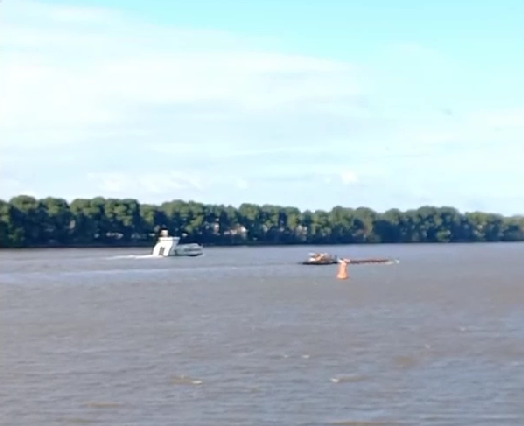
\includegraphics[width=\textwidth]{images/Evaluation/shiptracking_raw.png}
			\caption{Screenshot aus Beispieldatensatz Schiffstracking}
		\end{subfigure} \hfill
		\begin{subfigure}[b]{0.45\textwidth}
			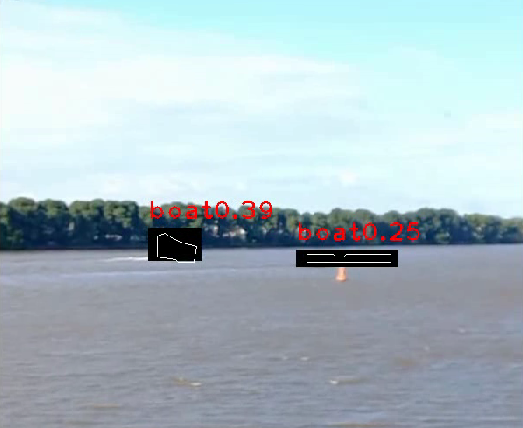
\includegraphics[width=\textwidth]{images/Evaluation/shiptracking_analyzed.png}
			\caption{Screenshot aus analysiertem Beispieldatensatz Schiffstracking}
		\end{subfigure}
		\caption[Screenshots zu Testdatensatz für Schiffstracking]{Screenshots zu Testdatensatz für Schiffstracking. (a) zeigt die Testdaten ohne Bearbeitung; (b) zeigt den Frame mit YOLO analysiert und von der DCE vereinfacht (Quelle: eigene Darstellung)}
		\label{Scr:Testdatensatz_Shiptracking}
	\end{figure} In Tabelle \ref{tab:Shiptracking_Analysis} ist der Vergleich der statistischen Daten zwischen den beiden verschieden langen Videos zu sehen. Auffällig ist, dass die durchschnittliche Abweichung pro Polygon deutlich absinkt, während die Abweichung pro Winkel steigt. Dies lässt sich mit den hohen Punktwerten nach der DCE erklären, aber auch damit, dass durch die Boje aus einem Schiff mehrere Schiffe von YOLO detektiert worden sind. Dies sorgt für eine hohe Abweichung, da die Boje den Umriss stark verfälscht. \\
	Die absolute Abweichung steigt bei dem längeren Video um ca. das 13-fache an. Dies kann mit der höheren Frameanzahl erklärt werden, wie auch die Zahl der erkannten Punkte/Winkel und Polygone, sowie der deutlich höheren Zahl der verglichenen Polygone. \\
	Die Prozessierungszeit von YOLO verdoppelt sich durch die höhere Framezahl, die Dauer der DCE steigt hingegen durch die erhöhte Anzahl von Polygonen deutlich stärker an. Beides ist dann auch in der Gesamtdauer des Programmes zu erkennen. \\
	Die SSM pro Klasse sinkt mit der höheren Framezahl ab, da mehr erkannte Polygone bei gleichbleibender Punktzahl zu einer Verringerung von diesem Wert führen. Dies ist auch deutlich bei der SSM pro detektiertes Boot zu erkennen, die ca. um die Hälfte verringert ist. \\

	\begin{table}[ht]
		\centering
		\caption[Auswertung Schiffstracking Datensatz]{Auswertung Schiffstracking Datensatz; S1s ist der 1-sekündige Datensatz, S21s ist der 21-sekündige Datensatz (Quelle: eigene Darstellung; \ref{cd:listing_A1s_RV_shiptracking_results.txt(Y8x)}, \ref{cd:listing_A21s_RV_shiptracking_results.txt(Y8x)})}
		\label{tab:Shiptracking_Analysis}
		\begin{tabular}{l|l|l|l}
			& \textbf{S1s\_Y8x} & \textbf{S21s\_Y8x} & \textbf{Faktor} \\ \hline
		   \textit{\begin{tabular}[c]{@{}l@{}}Durchschn. Abw.\\ p. Polygon (in Deg.)\end{tabular}} & 48,5 & 29,85 & 0,62 \\ \hline
		   \textit{\begin{tabular}[c]{@{}l@{}}Durchschn. Abw.  \\ p. Winkel (in Deg.)\end{tabular}} & 5,2 & 30,8 & 5,92 \\ \hline
		   \textit{} &  &  &  \\ \hline
		   \textit{\begin{tabular}[c]{@{}l@{}}absolute Abw. \\ (in Deg)\end{tabular}} & 2909,95 & 39109,72 & 13,44 \\ \hline
		   \textit{erk. Punkte/Winkel} & 560 & 12683 & 22,65 \\ \hline
		   \textit{erk.  Polygone} & 60 & 1310 & 21,83 \\ \hline
		   \textit{\begin{tabular}[c]{@{}l@{}}verglichene\\ Polygone\end{tabular}} & 49 & 1213 & 24,80 \\ \hline
			&  &  &  \\ \hline
		   \textit{\begin{tabular}[c]{@{}l@{}}Prozessierungszeit\\ (in Sek.)\end{tabular}} & 33,88 & \begin{tabular}[c]{@{}l@{}}738,25\\ (12,3 Min.)\end{tabular} & 21,80 \\ \hline
		   \textit{Dauer YOLO (in Sek)} & 30,09 & \begin{tabular}[c]{@{}l@{}}602,34\\ (10,04 Min.)\end{tabular} & 2,00 \\ \hline
		   \textit{Dauer DCE (in ms)} & 2,31 & 129,6 & 56,10 \\ \hline
			&  &  &  \\ \hline
		   \textit{SSM pro Fr. und Kl. Boot} & 229,32 & 133,15 & 0,06 \\ \hline
		   \textit{SSM pro detektiertes Boot} & 118,61 & 65,26 & 0,55 \\ \hline
		   \textit{\begin{tabular}[c]{@{}l@{}}Absolute Anz. detektierter\\ Boote (in Klam. pro Fr.)\end{tabular}} & \begin{tabular}[c]{@{}l@{}}58 \\ (1,93)\end{tabular} & \begin{tabular}[c]{@{}l@{}}1310\\ (2,04)\end{tabular} & \begin{tabular}[c]{@{}l@{}}22,59 \\ (1,06)\end{tabular}
		   \end{tabular}
		\end{table}
       \todo{Abschluss finden?}



}
\subsection{Geringe und hohe DCE Substitution}
	{ \todo{tabelen mit quellen versehen!}
		Bei diesem Testdaten werden die Fälle betrachtet, bei denen DCE geringere und höhere Punktgrenzen beachten muss. Als Referenz wird der 8x Datensatz in der Länge 1 Sekunde und in der Länge 10 Sekunden genutzt. Es wird immer die RV Version der Implementierung betrachtet. Die DCE Grenzen sind in Tabelle \ref{tab:YOLO8_minor_more_DCE_Limits} aufgelistet. \\
	\begin{table}[ht]
		\caption{Einstellungen der verschiedenen DCE Substitutionsgrenzen (Quelle: eigene Darstellung; \ref{cd:listing_A1s_RV_minor_results.txt(Y8x)}, \ref{cd:listing_A1s_RV_more_results.txt(Y8x)}, \ref{cd:listing_A10s_RV_minor_results.txt(Y8x)}, \ref{cd:listing_A10s_RV_more_results.txt(Y8x)})}
		\label{tab:YOLO8_minor_more_DCE_Limits}
		\centering
		\begin{tabular}{l|l|l|l}
		 & \textbf{\begin{tabular}[c]{@{}l@{}}Geringe DCE\\ Punktgrenzen\end{tabular}} & \textbf{Referenz} & \textbf{\begin{tabular}[c]{@{}l@{}}hohe DCE\\ Punktgrenzen\end{tabular}} \\ \hline
		\textit{Kl. Auto} & 5 & 10 & 60 \\ \hline
		\textit{Kl. Motorrad} & 3 & 5 & 25 \\ \hline
		\textit{Kl. LKW} & 4 & 8 & 40 \\ \hline
		\textit{anderes Objekt} & 5 & 20 & 100
		\end{tabular}
		\end{table}
		In Tabelle \ref{tab:YOLO8_minor_more_DCE_A1s} ist zu sehen, dass die durchschnittliche Abweichung pro Polygon und Winkel bei geringeren Punktgrenzen stark absinkt und bei höheren Punktgrenzen stark ansteigt. Dies kann man auch auf die absolute Abweichung und die erkannten Punkte übertragen. Da die Zahl der erkannten Punkte steigt, wenn die DCE weniger Punkte entfernt, steigen auch die anderen Werte. Dies gilt auch analog dafür, wenn die DCE mehr Punkte entfernt. \\
		Ein ähnliches Phänomen ist bei der Tabelle \ref{tab:Minor_More_DCE_SSMs_A1s} zu erkennen, wo die SSMs aufgelistet sind. Hier steigt die SSM massiv an, wenn DCE Grenzen angehoben werden und analog dazu sinkt die SSM, wenn die DCE Grenzen verringert werden. Dies ist gleichbleibend bei der absoluten Anzahl der beiden betrachteten Klassen Auto und LKW. \\
		Für die Ergebnisse bei dem 10-sekündigen Video siehe die Tabellen \ref{tab:Minor_More_DCE_SSMs_A10s} (S. \pageref{tab:Minor_More_DCE_SSMs_A10s})  und  \ref{tab:YOLO8_minor_more_DCE_A10s} (S. \pageref{tab:YOLO8_minor_more_DCE_A10s})  im Anhang. Diese Ergebnisse sind auf die oben beschriebenen übertragbar, außer das alle Werte deutlich ansteigen. \\

		\begin{table}[ht]
			\centering
			\caption{Vergleich der Statistik bei 1 Sekunde Video (30 Frames) und verschiedenen DCE Substitutionsgrenzen (Quelle: eigene Darstellung; \ref{cd:listing_A1s_RV_minor_results.txt(Y8x)}, \ref{cd:listing_A1s_RV_more_results.txt(Y8x)})}
			\label{tab:YOLO8_minor_more_DCE_A1s}
			\begin{tabular}{l|l|l|l}
				& \textbf{\begin{tabular}[c]{@{}l@{}}geringe DCE\\ Punktgrenzen\end{tabular}} & \textbf{Referenz} & \textbf{\begin{tabular}[c]{@{}l@{}}hohe DCE\\ Punktgrenzen\end{tabular}} \\ \hline
			   \textit{\begin{tabular}[c]{@{}l@{}}Durchschn. Abweichung\\ p. Polygon (in Deg.)\end{tabular}} & 3,08 & 48,12 & 454,81 \\ \hline
			   \textit{\begin{tabular}[c]{@{}l@{}}Durchschn. Abweichung  \\ p. Winkel (in Deg.)\end{tabular}} & 0,68 & 5,46 & 24,18 \\ \hline
			   \textit{} &  &  &  \\ \hline
			   \textit{\begin{tabular}[c]{@{}l@{}}absolute Abweichung  \\ (in Deg)\end{tabular}} & 658,93 & 10298,28 & 97329,43 \\ \hline
			   \textit{erkannte Punkte/Winkel} & 966 & 1885 & 4026 \\ \hline
			   \textit{erkannte Polygone} & 214 & 214 & 214 \\ \hline
			   \textit{verglichene Polygone} & 194 & 194 & 194 \\ \hline
			   \textit{Prozessierungszeit (in Sek.)} & 107,77 & 102,46 & 80,39
			   \end{tabular}
			\end{table}

			\begin{table}[ht]
				\caption{Vergleich der SSMs bei verschiedenen DCE Substitionslimits bei einem 1-sekündigem Video (30 Frames) (Quelle: eigene Darstellung; \ref{cd:listing_A1s_RV_minor_results.txt(Y8x)}, \ref{cd:listing_A1s_RV_more_results.txt(Y8x)})}
				\label{tab:Minor_More_DCE_SSMs_A1s}
				\centering
				\begin{tabular}{l|l|l|l}
				 & \textbf{\begin{tabular}[c]{@{}l@{}}geringe DCE\\ Punktgrenzen\end{tabular}} & \textbf{Referenz} & \textbf{\begin{tabular}[c]{@{}l@{}}hohe DCE\\ Punktgrenzen\end{tabular}} \\ \hline
				\textit{SSM pro Fr. und Kl. Auto} & 3,12 & 355,41 & 6638,88 \\ \hline
				\textit{SSM pro detektiertes Auto} & 0,90 & 102,52 & 1915,06 \\ \hline
				\textit{\begin{tabular}[c]{@{}l@{}}absolute Anz. detektierter\\ Autos (in Klam. pro Fr.)\end{tabular}} & 104 (3,47) & 104 (3,47) & 104 (3,47) \\ \hline
				 &  &  &  \\ \hline
				\textit{SSM pro Fr. und Kl. LKW} & 39,52 & 14,19 & 10388,78 \\ \hline
				\textit{SSM pro detektierter LKW} & 11,40 & 4,09 & 2996,76 \\ \hline
				\textit{\begin{tabular}[c]{@{}l@{}}absolute Anz. detektierter\\ LKW (in Klam. pro Fr.)\end{tabular}} & 104 (3,47) & 104 (3,47) & 104 (3,47)
				\end{tabular}
				\end{table}		
	 }
	 \clearpage
\subsection{lange Testdatensätze (NICHT FERTIG)}{
	\todo{müssen noch gemacht werden }
	
}
\subsection{Gleiche DCE Substitionslimits (NICHT FERTIG)}{
	\todo{müssen noch gemacht werden }}
{
	

}
% 	\section{Bewertung}
% 	{ %Zusammenfassen kann man sagen, dass die durchschnittliche Abweichung pro Polygon nach der Vereinfachung von DCE zu hoch ist, um ein Tracking zu ermöglichen. Beim Einsatz der größeren Modelle steigt die Winkelabweichung und SSM an, dies ist aber zu vernachlässigen, da die Klassifizierung der Objekte genauer erfolgt. Insbesondere der Vergleich der SSM innerhalb einer Klasse  ist die Abweichung sehr hoch. \\
% 	%Die Implementierung der YOLO Version in der Variante, dass das Video in einzelne Frames zerlegt wird und diese einzeln analysiert werden, hat sich im Vergleich zur direkten vollständigen Analyse mit YOLO als zu ineffektiv herausgestellt und kann damit verworfen werden. 
	
% 	Zusammenfassen kann man sagen, dass die durchschnittliche Abweichung pro Polygon nach der Vereinfachung von DCE gering genug ist, um ein Tracking zu ermöglichen. Beim Einsatz der größeren Modelle steigt die Winkelabweichung und SSM an, dies ist aber zu vernachlässigen, da die Klassifizierung der Objekte genauer erfolgt.  \\
% 	Die Implementierung der YOLO Version in der Variante, dass das Video in einzelne Frames zerlegt wird und diese einzeln analysiert werden, hat sich im Vergleich zur direkten vollständigen Analyse mit YOLO als zu ineffektiv herausgestellt und kann damit verworfen werden. }

% \section{Ausblick}
%  { 
% %	\begin{enumerate}
% % 	\item DCE Abbruchbedingung nicht fest implementieren sondern einen Wert einführen, der immer im Vergleich zur Ähnlichkeit des Ursprungspolygons gemessen wird. Ermöglicht eine bedarfsbezogene Vereinfachung des Polygons, individuell für jeden erkannten Umriss
% % 	\item Implementierung der DCE; bzw. anderer Programmteile in schnellerer Programmiersprache wie C/C++; bzw. hardwarenah(er)
% % \end{enumerate}
	


% }




\cleardoubleoddemptypage


%!TEX root = ../thesis.tex
\chapter{Fazit}
\label{ch:conclusion}

\Blindtext
\begin{definition}[\texorpdfstring{$\sigma$}-Algebra]
    Sei $X$ eine Menge. Eine Teilmenge $\Sigma \in \mathcal{P}\left(X\right)$ heißt
    $\sigma$-Algebra wenn die folgenden drei Eigenschaften gelten: 
    \begin{enumerate}
        \item $X \in \Sigma$
        \item $A \in \Sigma \implies X \setminus A \in \Sigma$
        \item $A_1,A_2,\dots \in \Sigma \implies A_1 \cup A_2 \cup \dots \in \Sigma$
    \end{enumerate}
\end{definition}
Für eine Liste von Umgebungen siehe \texttt{preamble.tex}


\cleardoubleoddemptypage

% when adding a new chapter comment out this line
%\input{chapter/chapterFile.tex}
%cleardoubleoddemptypage

\appendix % hier beginnt der Anhang
%!TEX root = ../thesis.tex
\chapter{Anhang}

\section{Listing mit Dokumentation und Kommentaren im Code}{\label{cd:gesamt_listing}}

%\lstset{commentstyle=\color{black}, stepnumber=2} 
\todo{More Comment auf Default setzen noch einbauen, oder doch oben kommentare nur weiß setzten nach lattenzaun}


\subsection{Main.py}{
    \lstinputlisting[caption={Main.py}, label = {cd:listing_main.py}]{../Code/main.py}}

\subsection{yolo\_every\_frame.py}{
    \lstinputlisting[caption={YOLO\_every\_frame.py}, label = {cd:listing_yolo_every_frame_py}]{../Code/YOLO/yolo_every_frame.py}}

\subsection{YOLO\_result\_version.py}{
    \lstinputlisting[caption={YOLO\_result\_version.py}, label = {cd:listing_yolo_result_version}]{../Code/YOLO/yolo_result_version.py}}

\subsection{YOLO\_segmentation.py}{
    \lstinputlisting[caption={YOLO\_segementation.py}, label = {cd:listing_yolo_segmentation.py}]{../Code/YOLO/yolo_segmentation.py}}

\subsection{DCE.py}{
    \lstinputlisting[caption={DCE.py}, label = {cd:listing_DCE.py}]{../Code/DCE/DCE.py}}

\subsection{Shape\_Similarity.py}{
    \lstinputlisting[caption={shape\_sim\_meas.py}, label = {cd:listing_shape_sim_meas.py}]{../Code/Shape_Similiarity/shape_sim_meas.py}
}


\cleardoubleoddemptypage

\listoffigures
\cleardoubleoddemptypage

\listoftables
\cleardoubleoddemptypage

\printbibliography
\cleardoubleoddemptypage
%!TEX root = ../thesis.tex
\chapter*{Plagiatserklärung des Studierenden}
Hiermit versichere ich, dass die vorliegende Arbeit über 
\begin{center}
\textit{\printtitle}
\end{center}
selbstständig von mir und ohne fremde Hilfe verfasst worden ist, dass keine anderen Quellen und Hilfsmittel als die angegebenen benutzt worden sind und dass die Stellen der Arbeit, die anderen Werken – auch elektronischen Medien – dem Wortlaut oder Sinn nach entnommen wurden, auf jeden Fall unter Angabe der Quelle als Entlehnung kenntlich gemacht worden sind. Mir ist bekannt, dass es sich bei einem Plagiat um eine Täuschung handelt, die gemäß der Prüfungsordnung sanktioniert werden kann.

\vspace{0.75cm}
\parbox{17em}{\hrulefill} \\
\printname, \printcity, 29.09.2023 \\
\vspace{0.5cm}



Ich erkläre mich mit einem Abgleich der Arbeit mit anderen Texten zwecks Auffindung von Übereinstimmungen sowie mit einer zu diesem Zweck vorzunehmenden Speicherung der Arbeit in einer Datenbank einverstanden. 

Ich versichere, dass ich die vorliegende Arbeit oder Teile daraus nicht anderweitig als Prüfungsarbeit eingereicht habe.



\vspace{0.75cm}
\parbox{17em}{\hrulefill} \\
\printname, \printcity, 29.09.2023




\end{document}
